% 可自定义论文时间戳 \today
\year=2021
\month=5
\day=20

\documentclass{sysuthesis} % 默认使用电子版(不填充空白页)。如果需要双面打印版,请注释掉本行并启用下一行
% \documentclass[print-both-sides]{sysuthesis} % 使用双面打印版(填充额外空白页以保证每一章开头都在奇数页)
\usepackage{sysucode}  % 在论文中使用代码

%%
% 论文相关信息
% 本文档中前缀"c-"代表中文版字段, 前缀"e-"代表英文版字段
% modifyer: 黄俊杰(huangjj27, 349373001dc@gmail.com)
% update date: 2017-04-13
%%

% 标题
% 论文题目应以简短、明确的词语恰当概括整个论文的核心内容,避免使用不常见的缩略词、缩写字。读者通过标题可大致了解毕业设计(论文)的内容、专业的特点和科学的范畴。中文题目一般不宜超过 24 个字,必要时可增加副标题。外文题目一般不宜超过 12 个实词

% 封面标题。由于技术所限,封面题目过长的划分交由用户您进行定夺
% 这也能让您的论文封面看起来更有美感
\covertitlefirst{中山大学}
\covertitlesecond{本科毕业论文(设计)}

% Author:   Souler Ou
% 修改者:    欧一锋
% Date:     3/30/2018
% Mail:     ou@souler.cc
%如果英文标题过长可以使用此两项作为表三(答辩记录表)的标题。
\etitlefirst{\LaTeX \ Template}
\etitlesecond{for SYSU Graduation Thesis}

% 中文标题
\ctitle{中山大学本科毕业论文}
\etitle{ \LaTeX \ Template for SYSU Graduation Thesis}

% 作者详细信息
\author{王小明}
\cauthor{王\ 小\ 明}    % 封面作者
\eauthor{Wang Xiaoming}
\studentid{12350004}
\cschool{计算机学院}

\cmajor{计算机科学与技术}
\emajor{Computer Science and Technology}

% 指导老师
\cmentor{王大明 \ (教授)}
\ementor{Prof. 王大明}

     % 论文相关信息
%%
% 开题报告
% modifier: 黄俊杰(huangjj27, 349373001dc@gmail.com)
% update date: 2017-05-14

% 选题目的
\objective{

}

% 思路
\methodology{

}

% 研究方法/程序/步骤
\researchProcedure{

}

% 相关支持条件
\supportment{

}

% 进度安排
\schedule{

}

% 指导老师意见
\proposalInstructions{

}

   % 开题报告内容
%%
% 摘要信息
% 本文档中前缀"c-"代表中文版字段, 前缀"e-"代表英文版字段
% 摘要内容应概括地反映出本论文的主要内容,主要说明本论文的研究目的、内容、方法、成果和结论。要突出本论文的创造性成果或新见解,不要与引言相 混淆。语言力求精练、准确,以 300—500 字为宜。
% 在摘要的下方另起一行,注明本文的关键词(3—5 个)。关键词是供检索用的主题词条,应采用能覆盖论文主要内容的通用技术词条(参照相应的技术术语 标准)。按词条的外延层次排列(外延大的排在前面)。摘要与关键词应在同一页。
% modifier: 黄俊杰(huangjj27, 349373001dc@gmail.com)
% update date: 2017-04-15
%%

\cabstract{

    随着单精度甚至更低精度浮点格式在现代AI应用中的普及,一个新基准HPL-AI被提出,以用于评估计算系统在混合精度计算场景上的性能。然而,该基准目前尚未有公开的通用实现。在本文中,我们实现了HPL-AI基准的首个开源的分布式实现,并在X86、CUDA、ARM64等多个平台对其正确性、通用性、可扩展性进行了测试。同时,我们将该实现移植到华为Atlas 800-9000训练服务器上,并针对其搭载的国产异构处理器华为昇腾910进行优化。实验结果表明,借助混合精度矩阵分解算法和数值迭代算法,我们的实现能获得与HPL相当甚至更高的计算精度,且带来显著性能提升。

}

% 中文关键词(每个关键词之间用“,”分开,最后一个关键词不打标点符号。)

\ckeywords{HPL-AI,MPI,混合精度,矩阵分解,数值迭代,华为昇腾910}

\eabstract{
    % 英文摘要及关键词内容应与中文摘要及关键词内容相同。中英文摘要及其关键词各置一页内。

    With the popularity of 32-bit and even lower floating-point precision formats in modern AI applications, a new benchmark, HPL-AI, was proposed to evaluate the performance of computing systems in mixed-precision scenarios. However, the benchmark currently had no publicly available general implementation. In this thesis, we completed the first open-source general MPI implementation of HPL-AI benchmark, and tested its correctness, versatility, and scalability on multiple platforms including X86, CUDA, and ARM64. Meanwhile, we transplanted the implementation to the HUAWEI Atlas 800-9000 training server, and optimized for domestic heterogeneous processors HUAWEI Ascend 910 on the server. Experimental results showed that with the help of the mixed-precision matrix factorization algorithm and iterative refinement algorithm, our implementation could obtain the accuracy equal to or even higher than that of HPL with a significant performance improvement.

}

% 英文文关键词(每个关键词之间用,分开, 最后一个关键词不打标点符号。)

\ekeywords{HPL-AI, MPI, mixed-precision, matrix factorization, iterative refinement, HUAWEI Ascend 910}
     % 摘要内容
%%
% 成绩评定记录表
% modifier: 黄俊杰(huangjj27, 349373001dc@gmail.com)
% update date: 2017-05-17

\gradingComment{
    某某同学针对什么问题研究了什么算法/实现了什么系统/针对这个系统做了什么测试,本文选题合理,实验结果表明技术路线……论文写作规范,引用文献充分,符合中山大学本科论文的规范,是篇优秀/良好/中等/合格的论文。
}
    % 成绩评定记录表评语
%%
% 四次进度报告相关信息

% Author:   Souler Ou
% 修改者:    欧一锋
% Date:     3/30/2018
% Mail:     ou@souler.cc

% 第一次进度报告
\firstsummary{
	\begin{adjustwidth}{2em}{2em}
		在这一阶段,XXX工作基本完成,主要在如下几个方面:
		\begin{enumerate}
			\item 完成了第一项。
			\item 完成了第二项
			\item 完成了第三项。
		\end{enumerate}
	\end{adjustwidth}
}
% 第2次进度报告
\secondsummary{
	\begin{adjustwidth}{2em}{2em}
		...
	\end{adjustwidth}
}
% 第3次进度报告
\thirdsummary{
	\begin{adjustwidth}{2em}{2em}
		...
	\end{adjustwidth}
}
% 第4次进度报告
\fourthsummary{
	\begin{adjustwidth}{2em}{2em}
		...
	\end{adjustwidth}
}
% 第1次老师评价
\firstcomment{
	\begin{adjustwidth}{2em}{2em}
		论文完成情况良好。
	\end{adjustwidth}
}
% 第2次老师评价
\secondcomment{
	\begin{adjustwidth}{2em}{2em}
		...
	\end{adjustwidth}
}
% 第3次老师评价
\thirdcomment{
	\begin{adjustwidth}{2em}{2em}
		...
	\end{adjustwidth}
}
% 第4次老师评价
\fourthcomment{
	\begin{adjustwidth}{2em}{2em}
		...
	\end{adjustwidth}
}
% 老师总评价
\finalcomment{
	\begin{adjustwidth}{2em}{2em}
		...
	\end{adjustwidth}
}   % 过程检查报告数据
\begin{document}
% 论文前置部分
\frontmatter
\pagenumbering{Roman}
\makeUndergraduateCover    % 封面
\makeUndergraduateTitlePage    % 扉页
% \makeProposal% 开题报告
% \makeProgressCheck  % 过程检查记录表
% \makeDefenseRecord  % 答辩情况等级表
\makedisclaim       % 学术诚信声明
\makeabstract       % 中英文摘要
\maketableofcontents        % 目录
\makelistoffiguretable

% 论文主体部分
\mainmatter
% 引言

% 正文
%%
% 引言或背景
% 引言是论文正文的开端,应包括毕业论文选题的背景、目的和意义;对国内外研究现状和相关领域中已有的研究成果的简要评述;介绍本项研究工作研究设想、研究方法或实验设计、理论依据或实验基础;涉及范围和预期结果等。要求言简意赅,注意不要与摘要雷同或成为摘要的注解。
% modifier: 黄俊杰(huangjj27, 349373001dc@gmail.com)
% update date: 2017-04-15
%%

\chapter{绪论}
%定义,过去的研究和现在的研究,意义,与图像分割的不同,going deeper
\label{cha:introduction}
\section{选题背景与意义}
\label{sec:background}
% What is the problem
% why is it interesting and important
% Why is it hards, why do naive approaches fails
% why hasn't it been solved before
% what are the key components of my approach and results, also include any specific limitations,do not repeat the abstract
%contribution
引言是论文正文的开端,应包括毕业论文选题的背景、目的和意义;对国内外研究现状和相关领域中已有的研究成果的简要评述;介绍本项研究工作研究设想、研究方法或实验设计、理论依据或实验基础;涉及范围和预期结果等。要求言简意赅,注意不要与摘要雷同或成为摘要的注解。

\section{国内外研究现状和相关工作}
\label{sec:related_work}
对国内外研究现状和相关领域中已有的研究成果的简要评述。
\section{本文的论文结构与章节安排}

\label{sec:arrangement}

本文共分为六章,各章节内容安排如下:

第一章绪论。简单说明了本文章的选题背景与意义。

第二章为本科生毕业论文写作与印制规范。本章节就学校的规范,逐点进行描述,并给出来了相关例子说明本模板在格式上的正确性。

第三章为本模板的使用说明。

第四章为可用的\LaTeX 的代码段方便大家进行编辑。

第五、六章是本文的最后两章,作为空白章节例子。


\newclearpage
\chapter{HPL-AI算法分析与实现}

\label{HPL-AI算法分析与实现}

\section{HPL-AI基准规则}

根据HPL-AI的主页\cite{dongarrahpl},我们归纳了这一新基准的主要思想,主要包括以下两点:

\begin{enumerate}
    \item 对矩阵进行混合精度分解,然后计算较低精度分解下得到的近似解。
    \item 使用前一步得到的解作为预条件(preconditioner),使用 64 位精度的迭代方法(如 GMRES)迭代,最终得到与 64 位精度 LU 分解相当的精确度。
\end{enumerate}

\subsection{矩阵构造}

基准的实现应当参照 HPL,但需要修改矩阵生成器:应当构造一个非对称的对角优势(diagonally dominant)矩阵,可以保证用直接法或迭代法解线性代数方程组的稳定性和收敛性。

\subsection{混合精度}

分解过程可以使用混合精度,例如:panel 分解和三角矩阵求解可以用 32 位精度完成,舒尔补充过程(Schur complement,即$A_{2,2} \leftarrow A_{2,2} - A_{2,1} \times A_{1,1}^{-1} \times A_{1,2}$ 形式的矩阵乘法)可以用 32 位累加的 16 位精度来计算。

为了在所有计算机上实现一致的性能标准,在基准测试过程中求解低精度方程组时使用的算法必须在数学上等价于 LU 因式分解,且所需的浮点操作数(即使不需要双精度运算)必须是 $\frac{2}{3} n^3 + \frac{3}{2} n^2$(LU 因式分解需要 $\frac{2}{3} n^3 - \frac{1}{2} n^2$,$2n^2$ 用于随后的后向和正向求解)。

同时,HPL-AI允许在浮点格式范围内对结果进行平衡缩放,但所需的时间必须包含在求解时间中。

\subsection{误差与限制}

HPL-AI的误差由此式确定:
$$
    \frac{\Vert Ax-b\Vert_{\infty}}{\Vert A\Vert_{\infty} \Vert x\Vert_{\infty} + \Vert b\Vert_{\infty}} \times (n \times \epsilon)^{-1}
$$
其中,$n$ 是输入矩阵的大小;$\epsilon$ 是 64 位浮点算术中的机器精度,在 IEEE 标准下有 $\epsilon=2^{−53}\approx 1.1\times 10^{-16}$。

HPL-AI的规则对 $n$ 没有限制,但数值迭代至多不能超过50轮,且其得到的最终误差必须小于 $16$。

\subsection{提交结果}

HPL-AI的计算效率基于计算系统求解问题的时间总和:较低精度矩阵分解过程、(可能的)防止溢出的平衡放缩过程、执行 GMRES 或使用 LU 因子作为预条件的使用 64 位浮点运算的其他迭代过程。在计算效率时,用$\frac{2}{3} n^3 + \frac{3}{2} n^2$除以总的解算时间,得到每秒的运算速率。

作为提交结果的一部分,提交者被希望提供提交中使用的算法的详细说明。

\section{矩阵生成器}

\autoref{matA}给出我们构造的矩阵在数学上的描述,其中$\alpha,\beta$为矩阵的构造参数,可通过\cite{2021Matrices}中的方法选取。此处我们我们设置条件数$\kappa=100$,比例系数$\rho=0.5$,则有$\beta=2.50/N,\alpha=\rho\beta=1.25/N$。同时,我们也使用了来自\cite{2021Matrices}的系数$\psi=f_{\max}/2=65504/2$对矩阵进行缩放,使得该矩阵可以在FP16精度下被安全分解。

\begin{equation}
    \left(A\left(\alpha,\beta\right)\right)_{i,j}=\begin{cases}
        -\alpha+\left(j-1\right)\alpha\beta & \text{if } i>j \\
        1+\left(i-1\right)\alpha\beta       & \text{if } i=j \\
        -\beta+\left(i-1\right)\alpha\beta  & \text{if } i<j \\
    \end{cases}\label{matA}
\end{equation}

根据\cite{2021Matrices}中的证明,$\psi A\left(\alpha,\beta\right)$可以在$O(n^2)$的浮点操作内构造,且不需要选取主元即可稳定LU分解,符合HPL-AI基准要求.

\section{LU分解算法}

我们基于 HPL 软件包的实现,使用 LU 分解方法求解线性方程组。LU 分解存在三种方法,right-looking,left-looking 和 crout-looking,此处采用的是更容易被并行化的 right-looking 的分解方法\cite{2013Correcting}。\autoref{equ:right-looking} 给出right-looking LU分解的数学描述。

\begin{equation}
    \label{equ:right-looking}
    \begin{bmatrix}
        A_{1,1} & A_{1,2} \\
        A_{2,1} & A_{2,2}
    \end{bmatrix}
    =
    \begin{bmatrix}
        L_{1,1} & 0       \\
        L_{2,1} & L_{2,2}
    \end{bmatrix}
    \begin{bmatrix}
        U_{1,1} & U_{1,2} \\
        0       & U_{2,2}
    \end{bmatrix}
\end{equation}

以下是具体分解顺序:

\begin{wrapfigure}{r}{0.3\linewidth}
    \centering
    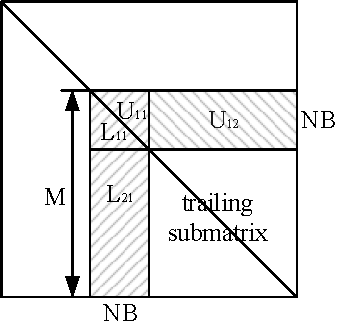
\includegraphics[width=0.3\textwidth]{image/chap02/LU}
    \caption{对输入矩阵 A 进行 LU 分解的示意图}
    \label{对输入矩阵 A 进行 LU 分解的示意图}
\end{wrapfigure}

\begin{enumerate}
    \item $A_{1,1} \leftarrow L_{1,1} U_{1,1},A_{2,1} \leftarrow L_{2,1}U_{1,1}$
    \item $A_{1,2} \leftarrow L_{1,1} U_{1,2}$
    \item $A_{2,2} \leftarrow A_{2,2} - L_{2,1}U_{1,2}$
    \item $A_{2,2} \leftarrow L_{2,2}U_{2,2}$
\end{enumerate}

\autoref{对输入矩阵 A 进行 LU 分解的示意图} 给出了对输入矩阵进行分解的示意图。分解过程中,每次循环迭代分解一个 $M\times\mathit{NB}$ 的矩阵,这个被分解的 $\mathit{NB}$ 列矩阵称之为 panel,$\mathit{NB}$ 是算法的输入参数,在输入文件 \lstinline{HPL.dat} 中指定。第一步是对 $\mathit{NB}$ 列、$M$ 行的矩阵进行分解,得到 $L_{1,1}$、$U_{1,1}$ 和 $L_{2,1}$,这一步称之为 panel 分解(panel factorization),在分解过程中,同时会执行 panel 内的选主元操作,并将结果进行保存;第二步进行三角矩阵求解(trsm),得到 $U_{1,2}$;第三步
    是对 $(M-\mathit{NB}) \times (M-\mathit{NB})$ 的剩余子矩阵(trailing submatrix)进行更新(gemm),得到待分解的 $L_{2,2}U_{2,2}$。

    通过如上三个步骤,成功把输入矩阵求解的问题转换成剩余子矩阵 $\leftarrow L_{2,2}U_{2,2}$ 的求解问题。于是,后续迭代只需要对重复对剩余子矩阵应用上述三个步骤,即可完成对整个问题的求解。

    \subsection{LU分解的并行化}
    \label{LU分解的并行化}

    \begin{wrapfigure}{r}{0.5\linewidth}
        \centering
        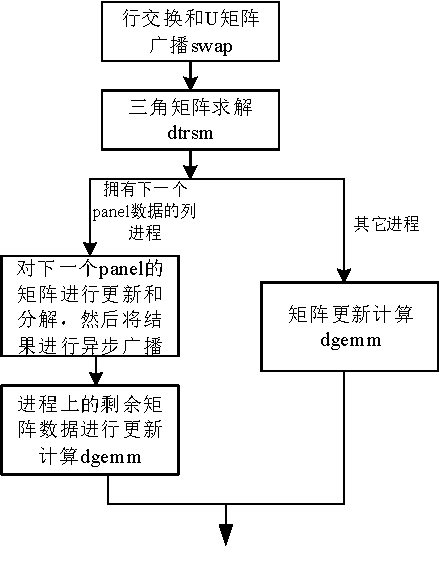
\includegraphics[width=0.5\textwidth]{image/chap02/PLU}
        \caption{并行LU分解的基本步骤图}
        \label{并行LU分解的基本步骤图}
    \end{wrapfigure}

    我们沿用了来自HPL的并行LU分解算法,\autoref{并行LU分解的基本步骤图}给出了该算法的基本步骤图。我们将所有参与计算的$\mathit{np}$个进程组织成一个二维的$P\times Q$进程网格,以$\mathit{NB}\times\mathit{NB}$为单位block-cyclic的方式均匀映射到输入矩阵$A$;$P,Q,\mathit{NB}$等是算法的输入参数,进程排列可选row-major和column-major两种方式。Panel分解完成后,panel所在的列进程将分解后的结果进行广播。然后,在剩余子矩阵中进行行交换,并广播U矩阵,这一步称之为swap。随后,在每个进程上进行trsm的计算过程。最后一步,对剩余子矩阵进行矩阵更新操作。

    \autoref{输入矩阵在进程间的分配图}给出了row-major映射下$P=2,Q=4$时,进程分布和输入矩阵在进程间的数据分配图,阴影部分数据为当前panel,其所在的列进程为5和1号进程,panel广播操作是5号进程将其所有的当前panel的分解结果广播给其它的行进程,即6、7和4号进程;同时,1号进程将其所有的panel分解结果广播给予其在同一行的进程,即2、3和0号进程。U矩阵广播操作是6号进程将其所有的U矩阵广播给予其在同一列上的2号进程,同时,7和4号进程也将其所有的U广播给予其在同一列的进程。

    \begin{wrapfigure}{r}{0.3\linewidth}
        \centering
        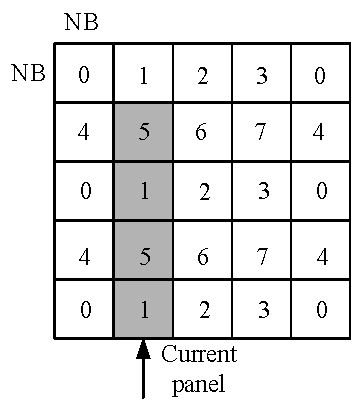
\includegraphics[width=0.3\textwidth]{image/chap02/LUP}
        \caption{输入矩阵在进程间的分配图}
        \label{输入矩阵在进程间的分配图}
    \end{wrapfigure}

    注意到Panel广播和矩阵更新没有依赖关系,可以并发执行以隐藏广播开销,这也是来自HPL中的一种通信优化方法,被称作Lookahead。拥有下一个Panel的列进程步骤是:首先,对下一个panel的矩阵数据进行更新计算,然后,对更新结果进行panel分解,并将分解结果在行向进行异步广播,最后,更新进程上的剩余子矩阵。同时,所有的其它进程进行当前剩余子矩阵的更新计算。这样就实现了下一个panel的广播和当前剩余子矩阵更新计算的重叠。

    \subsection{Panel分解}

    Panel分解是整个LU分解计算的关键步骤\cite{2013Correcting},拥有当前panel数据的所有列进程参与分解计算。三种LU分解算法均可用于panel分解,并可由输入参数中的recursive panel fact参数指定:left-looking、right-looking和crout-looking。这三种算法都是以递归方式实现的,递归分解的粒度根据输入参数中的$\mathit{NBMIN}$和$\mathit{NDIV}$两个参数控制:$\mathit{NBMIN}$是递归算法的停止条件,指定了进行分解的最少列数;$\mathit{NDIV}$是用于确定每个panel被划分成子panel的数目。当前Panel的$\mathit{NB}$列矩阵每次以$\mathit{NDIV}$份进行递归的列划分,直到最小列$\mathit{NBMIN}$。

    接下来我们以$\mathit{NB}=256,\mathit{NBMIN}=8,\mathit{NDIV}=4$的参数为例,对三种panel分解算法流程进行描述。256列的panel首先被分成4个subpanel,每个subpanel是64列的矩阵,在后面的描述中以subp 1, subp 2等代替。由于$64>\mathit{NBMIN}$,因此,每个64列的矩阵继续被分成4个subpanel,每个subpanel是16列。由于$16/\mathit{NDIVs}=4<\mathit{NBMIN}$,所以无法再对16列的subpanel进行划分,得到的最小subpanel的列数为16。最小的subpanel在后面的描述中分别以subp a, subp b等代替。

    \subsubsection{left-looking}

    \begin{wrapfigure}{r}{0.5\linewidth}
        \centering
        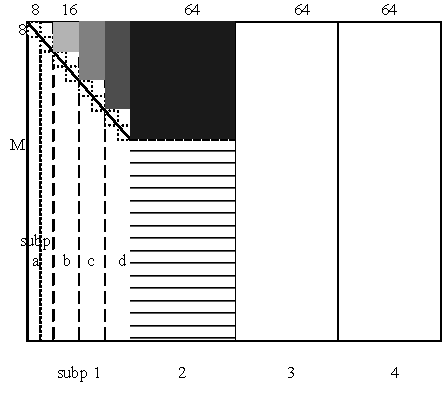
\includegraphics[width=0.5\textwidth]{image/chap02/left-looking}
        \caption{left-looking分解算法}
        \label{left-looking分解算法}
    \end{wrapfigure}

    \autoref{left-looking分解算法}给出left-looking分解算法图示。首先,对subp a进行分解;然后,进行dtrsm计算,得到subp b中的U矩阵(阴影部分);随后,利用subp a中的矩阵和U矩阵更新subp 中的trailing submatrix;最后,对更新后的subp b的trailing submatrix进行分解计算,这样就完成了subp b的分解计算。按照同样的步骤完成对subp c和subp d的计算工作。这样,就完成了对subp 1的分解计算。接下来,进行trsm计算得到subp 2的U矩阵,并对subp 2的trailing submatrix进行更新计算。随后,对subp 2的分解计算步骤和subp 1的分解步骤完全相同。按照这种递归方法,完成对subp 3和subp 4的分解计算,就完成了对整个panel的分解计算。

    \subsubsection{crout-looking}

    \begin{wrapfigure}{r}{0.5\linewidth}
        \centering
        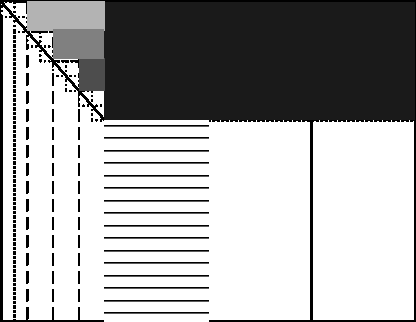
\includegraphics[width=0.5\textwidth]{image/chap02/crout-looking}
        \caption{crout-looking分解算法}
        \label{crout-looking分解算法}
    \end{wrapfigure}

    \autoref{crout-looking分解算法}给出crout-looking分解算法图示。首先,对subp a进行分解;然后,进行trsm计算,得到subp 1中$16\times48$的U矩阵(subp 1中最上层的阴影部分);随后,对subp b中的$(M-16)\times16$的trailing submatrx进行更新;最后,对subp b进行分解计算,这样就完成了subp b的分解计算。按照同样的步骤,完成subp c和subp d的分解计算。接下来,进行trsm计算得到整个panel的一个$64\times192$的U矩阵,并对subp 2的$(M-64)\times64$的trailing submatrix进行更新计算。以此递归方式完成对完成了对整个panel的分解计算。

    \subsubsection{right-looking}

    \begin{wrapfigure}{r}{0.5\linewidth}
        \centering
        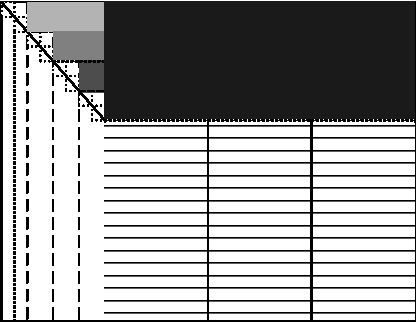
\includegraphics[width=0.5\textwidth]{image/chap02/right-looking}
        \caption{right-looking分解算法}
        \label{right-looking分解算法}
    \end{wrapfigure}

    \autoref{right-looking分解算法}给出right-looking分解算法图示。首先,对subp a进行分解;然后,进行trsm计算,得到subp 1中$16\times48$的U矩阵(subp 1中最上层的阴影部分);随后,对subp 1中的$(M-16)\times48$的trailing submatrx进行更新;最后,对subp b进行分解计算,这样就完成了subp b的分解计算。按照同样的步骤,完成subp c和subp d的分解计算。接下来,进行trsm计算,得到剩余panel的一个$64\times192$的U矩阵,并对整个panel的$(M-64)×192$的trailing submatrix进行更新计算。以此递归方式完成对完成了对整个panel的分解计算。

    \section{数值迭代算法}

    在问题求解的IR阶段,我们参照了来自HPL-AI主页实现的GMRES算法(Generalized Minimal Residual,广义最小残差算法)\cite{1986GMRES},并将其扩展到与HPL相同进程分布的MPI实现,尽可能减少数据重组和额外通信。GMRES是一种求解形如$Ax=b$线性形式方程的高效迭代算法。利用Arnoldi迭代法,将线性方程转化为一个线性最小二乘法的问题,再最小化这个残余量矢量,从而通过初始解$x_0$求出$x$在Krylov子空间的近似解。

    \subsection{Householder变换}

    传统GMRES使用Arnoldi算法将矩阵转换为Hessenberg矩阵,并利用Givens旋转法对Hessenberg矩阵进行处理。虽然这是最经典的方法,但是稳定性不够高,在实验中我们发现其容易使得GMRES收敛慢。

    因此,我们使用了Householder变换代替Arnoldi算法的格拉姆-施密特正交化过程,通过额外引入少量计算得到更加稳定的结果。\cite{1988Implementation}给出了使用Householder变换的GMRES算法的完整流程及数学证明,\autoref{使用Householder变换的GMRES算法}是该算法的伪代码。

    \begin{algorithm}[h]
        \KwIn{初始解$x_0$,容错值$\mathit{TOL}$,迭代轮数$\mathit{MAXIT}$}
        初始化:$L_1=(1),U_1=(u_1),r_0=b-Ax_0$\;
        确定$P_1$使得$P_1r_0=\pm\lVert r_0\rVert_2e_1$\;
        \ForEach{$m=1,2,\dots,\mathit{MAXIT}$}{
        计算$v\equiv \lbrace I-2U_mL_m^{-1}U_m^T\rbrace A \lbrace I-2U_m(L_m^T)^{-1}U_m^T\rbrace e_m$\;
        \If{$v^{(m+1)}=\dots=v^{(n)}=0$不满足}{
        计算$P_{m+1}=I-2u_{m+1}u_{m+1}$,其中$u_{m+1}$的前$m$个组分为零,这样$P_{m+1}v$在第$(m+1)st$之后具有零组分\;
        更新$v\leftarrow P_{m+1}v$\;
        }
        \If{$m>1$}{更新$v\leftarrow J_{m-1}\dots J_1v$}
        \If{$v^{(m+1)}\neq0$}{
            确定用于组分$m,m+1$的$J_m$,使得$\left(J_mv\right)^{\left(m+1\right)}=0$\;
            更新$v\leftarrow J_mv,w\leftarrow J_mw$\;
        }
        设置$R_m=\begin{cases}
                \left(v\right)         & \text{if } m=1 \\
                \left(R_{m-1},v\right) & \text{if } m>1
            \end{cases}$\;
        \If{$m<\mathit{MAXIT}$且$\lvert w^{(m+1)}\rvert>\mathit{TOL}$}{
            计算$L_{m+1}=\begin{bmatrix}
                    L_m           & 0 \\
                    2u_{m+1}^TU_m & 1
                \end{bmatrix}$;
            计算$U_{m+1}=\begin{bmatrix}U_m & u_{m+1}\end{bmatrix}$\;
        }
        \Else{
            求解$R_m$的上三角矩阵作为系数矩阵、$w$作为右手列的线性方程组,得到使得$\lVert 2-R_my\rVert_2$最小的$y_m$\;
            更新$x_0\leftarrow x_0+\lbrace I-2U_m\left(L_m^T\right)^{-1}U_m^T\rbrace\left(e_1,\dots,e_m\right)y_m$\;
            \If{$\lvert w^{(m+1)}\rvert>\mathit{TOL}$}{
                以当前的$x_0$作为输入,重新递归进行本算法\;
            }
            退出算法,返回结果$x_0$\;
        }
        }
        \caption{使用Householder变换的GMRES算法}
        \label{使用Householder变换的GMRES算法}
    \end{algorithm}

    值得注意的是,$\mathit{TOL}$是不同于HPL-AI算法的误差值的一个参数。

    \subsection{运行策略}
    \label{运行策略}

    GMRES 的主要缺点是:每次迭代所需的时间复杂度和空间复杂度会随着迭代次数的上升而增加。因此,除非(幸运地)很快就能够收敛,计算代价将迅速变得令人望而却步。

    克服这种限制的通常方法是重启迭代。在选定的迭代次数$m$之后,清除累积数据,中间结果被用作下一次迭代的初始数据;重复此过程,直到自身的误差值$<\mathit{TOL}$。不幸的是,$m$的选取没有明确的规则,这是一个经验问题。$m$过大,算法的时间和空间开销会超过起来来的收益;$m$过小,难以得到足够收敛的结果。

    与HPL-AI参考实现相同,我们使用$m=50$,并将GMRES自身的容错值设置成$\mathit{TOL}=\epsilon/2.0/(n/4.0)$。其中,$n$ 是输入矩阵的大小;$\epsilon$ 是 64 位浮点算术中的机器精度,在 IEEE 标准下有 $\epsilon=2^{−53}\approx 1.1\times 10^{-16}$。

    与参考实现不同的是,为减少运行时的开销,我们并没有在每轮迭代之后检查HPL-AI自身的误差。当然,从理论上来说,此处的参数选择有可能导致返回的结果误差超过HPL-AI的限制(例如当$N/\mathit{NB}$的比值不合理,导致浮点数的累加误差增大)。但根据我们的实验结果,在$N\sim 10^{5}$的时候,我们的实现可以在大部分情况下得到收敛的结果,并相对于LU分解过程有极小的开销。

此外我们甚至发现,在ARM64环境下链接到 openblas@0.3.8 及以下版本并开启OpenMP支持时,因其存在的多线程race的bug,HPL会概率返回错误的运行结果\footnote{详见\url{https://github.com/wu-kan/HPL-AI/issues/1},解决方法见\autoref{软件依赖}};而此时HPL-AI使用了数值迭代,反而可以返回正确的值。这说明我们的GMRES实现及其参数选择有很高的鲁棒性。

\section{面临的挑战}

结合上述分析,要针对一个计算系统实现高性能的HPL-AI基准,需要面临如下挑战,这也是我们在\autoref{面向国产异构处理器的移植工作}中致力于解决的目标。


\subsection{针对硬件的混合精度算法设计}

现代的硬件平台通常针对新兴的AI应用提供了包括FP16、BF16在内的多种计算精度支持\footnote{\url{https://nhigham.com/2018/12/03/half-precision-arithmetic-fp16-versus-bfloat16/}},他们的性能通常远优秀于传统HPC应用中使用的FP64、FP32。

因此,需要结合具体硬件规格,在不同计算阶段选用不同的精度和计算设备。例如,可以在panel分解和三角矩阵求解中使用FP32在CPU完成,在矩阵乘法更新剩余子矩阵过程中使用FP16/BF16/TF32在异构处理器上完成。同时,也需要考虑引入额外的放缩过程/数值迭代过程,减少/恢复计算过程中的精度损失。

\subsection{异构计算中的负载均衡问题}

目前主流的超算系统均为异构系统,在通用CPU之外同时搭载高性能的异构处理器用于处理专用问题。这类系统通常需要由CPU将任务传输到异构处理器上,并且等待异构处理器将任务完成。

因此,由此引入的任务传输开销及负载问题仍然是需要考虑的。例如,可以使用CPU负载部分任务,在减少异构处理器的负载同时掩盖CPU和异构处理器的传输开销。

\subsection{高性能的BLAS和MPI过程实现}

HPL/HPL-AI中包含了大量线性代数过程调用,其计算的绝大部分是gemm和trsm两个关键步骤,其性能取决于BLAS库(Basic Linear Algebra Subprograms)的性能\cite{endo2010linpack}。根据实验中的经验,本质为矩阵乘法的剩余矩阵更新占据了主要计算时间的80\%以上。此外,计算系统中进程间的通信问题同样会极大影响整体运算的效率,而HPL/HPL-AI中的通信过程一般通过MPI标准实现。

因此,针对计算系统实现的HPL-AI基准应当包含高效的BLAS和MPI实现,并且应当针对硬件架构和计算过程中的各种问题规模进行调优,以充分利用整个系统的算力。

\newclearpage
\chapter{\LaTeX 模板配置与使用}


\label{cha:sysu-thesis-latex-install-guide}

本部分内容将让你能够通过本\LaTeX 模板生成一份可用的pdf,并为后面修改源码撰写毕设做准备。

首先,我们会展示最简单的方法:直接使用overleaf进行编写。然后,我们整理了不同环境下\LaTeX 环境的配置指南与不同写作工具的配置技巧,方便各位同学使用本\LaTeX 模板。最后,我们说明了如何开始编写自己的毕业论文(设计)。


\section{使用Overleaf编写毕设}

Overleaf\footnote{网址可见\url{https://www.overleaf.com/}}是一个在线的Latex文档协作平台。我们不需要配置任何环境,便能够在上面直接使用本模板进行写作。操作步骤如下:

第一步,下载本项目压缩包(从\url{https://github.com/SYSU-SCC/sysu-thesis/releases}处下载即可),注意需要下载zip格式的压缩包。
然后,我们在Overleaf上新建项目,并上传该压缩包,可参考\autoref{fig:overleaf-new-proj}。


\begin{figure}[h]
	\centering
	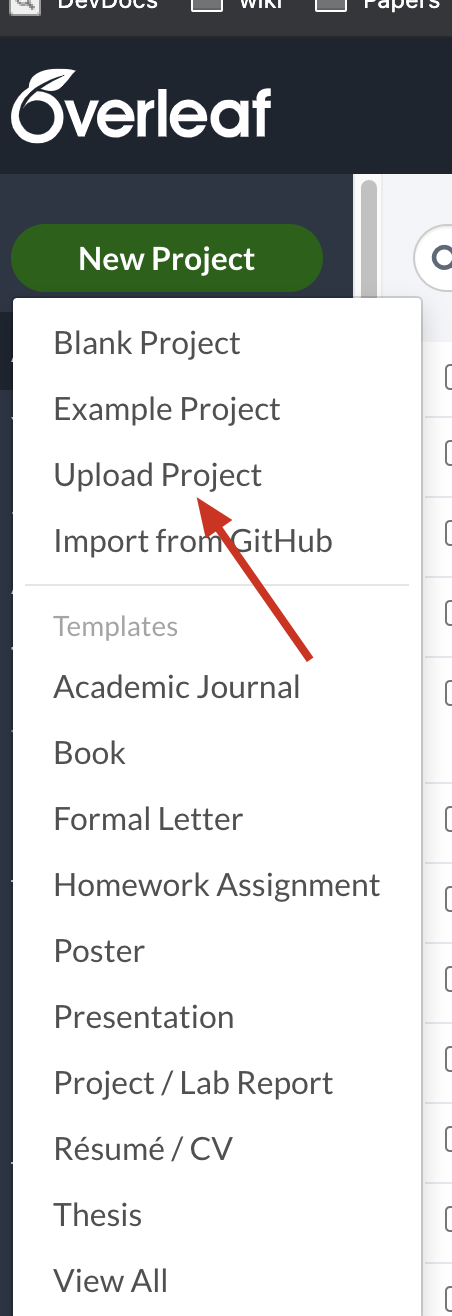
\includegraphics[width=0.2\textwidth]{image/chap03/overleaf-create-proj.jpg}
	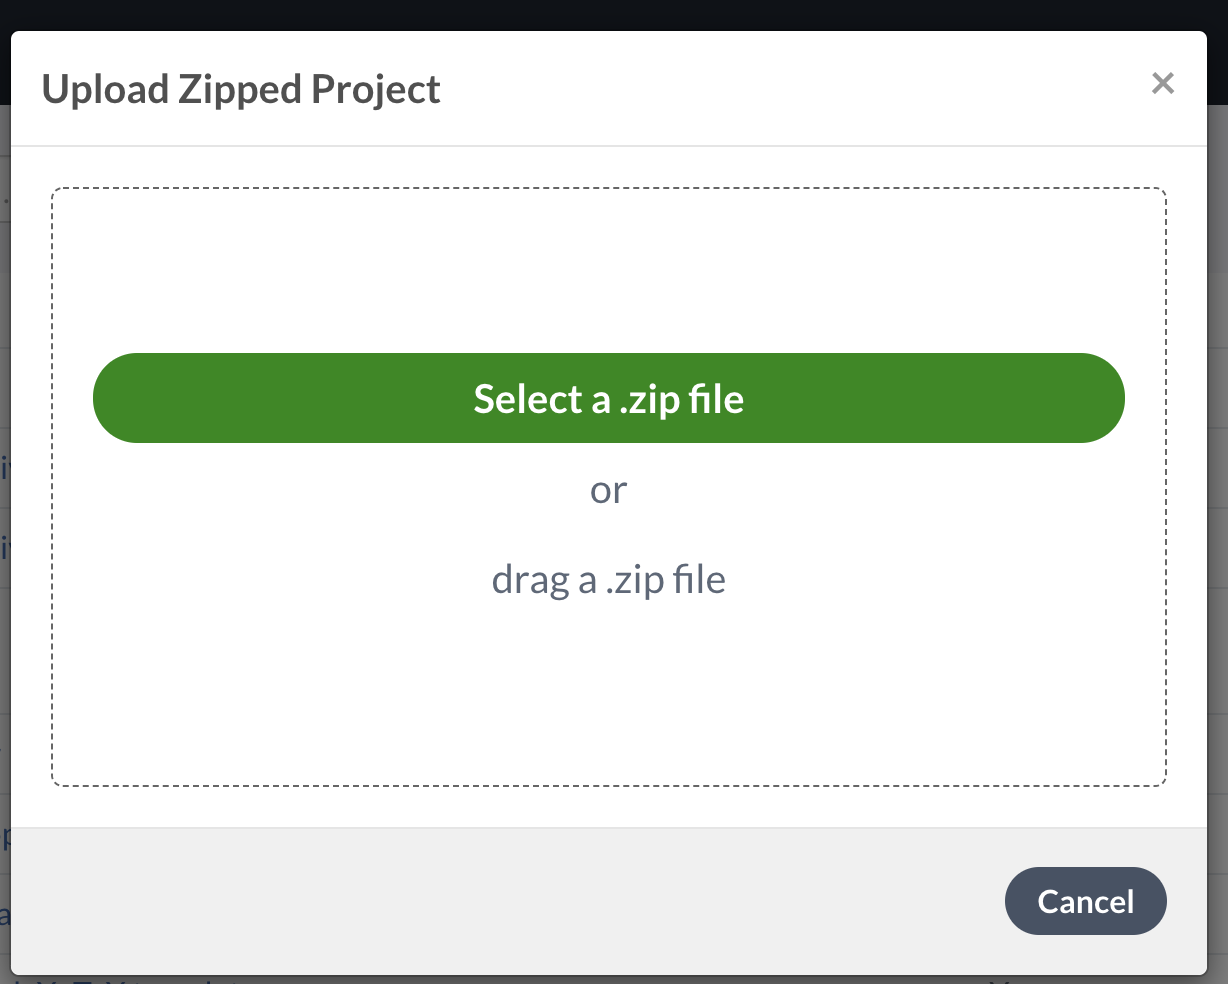
\includegraphics[width=0.7\textwidth]{image/chap03/overleaf-upload-proj.jpg}
	\caption{在Overleaf上创建并上传压缩包。}
	\label{fig:overleaf-new-proj}
\end{figure}

第二步,在Overleaf的菜单中调整编译工具为\texttt{xelatex},可参考\autoref{fig:overleaf-config}。

\begin{figure}[h]
	\centering
	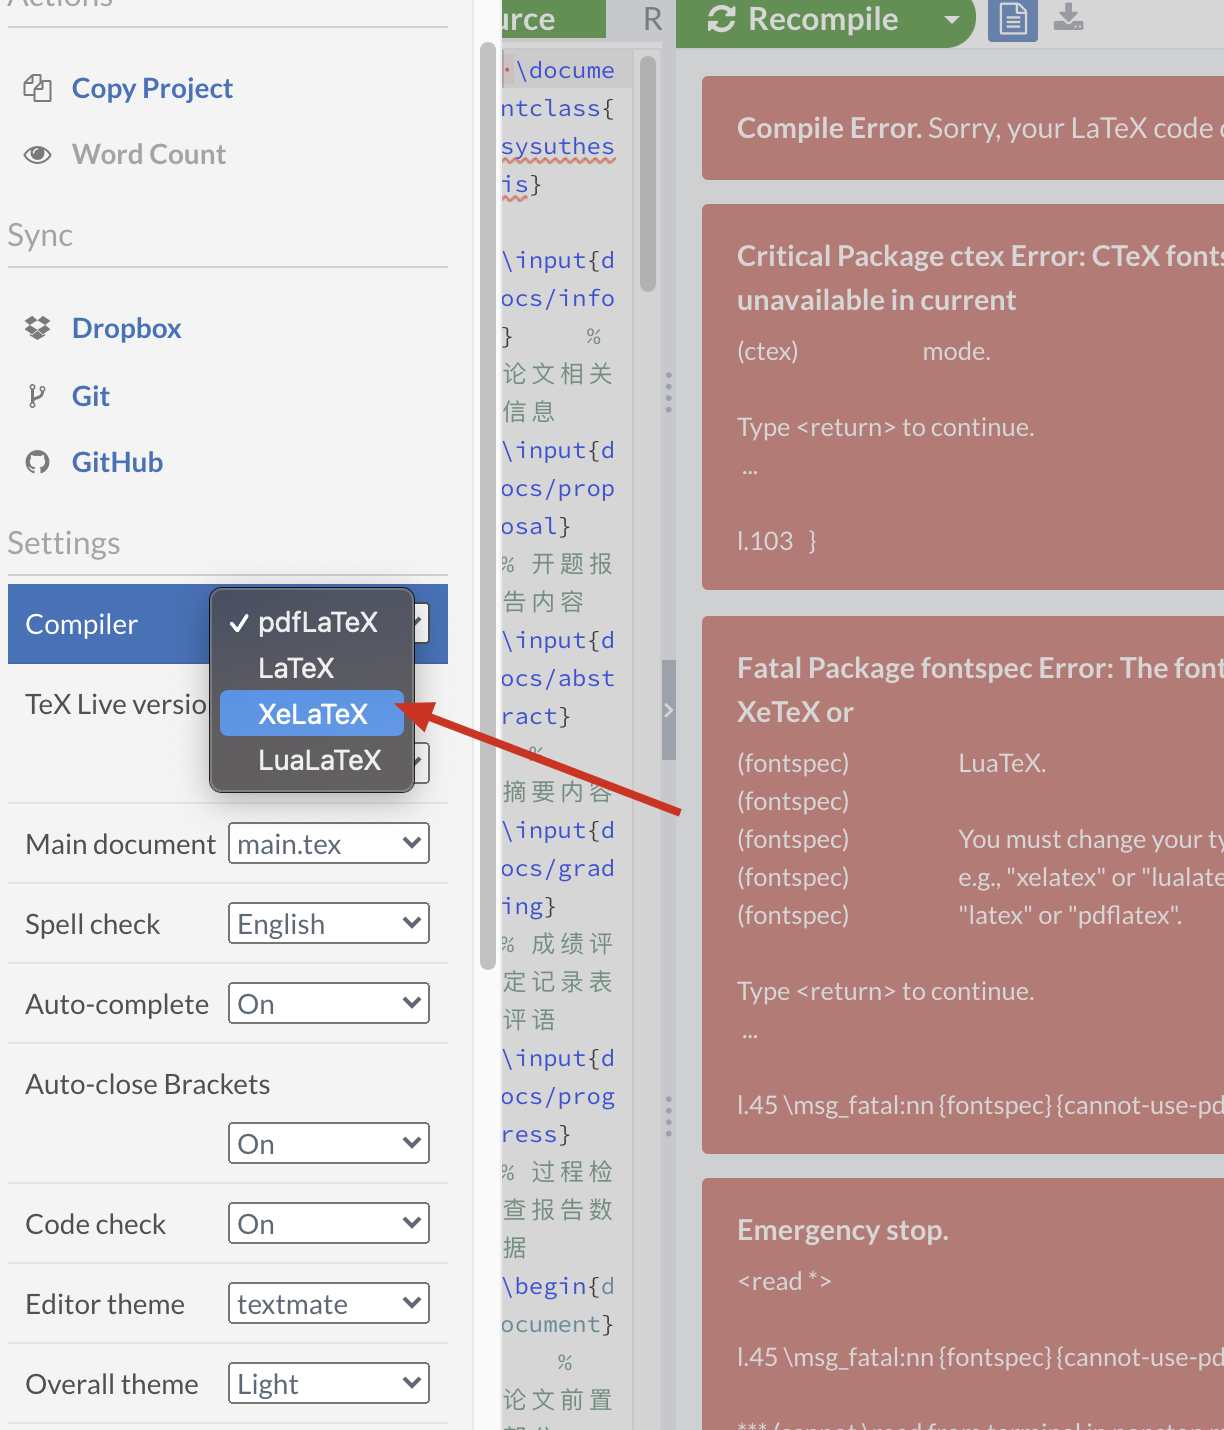
\includegraphics[width=0.6\textwidth]{image/chap03/overleaf-config.jpg}
	\caption{在Overleaf上调整编译工具}
	\label{fig:overleaf-config}
\end{figure}


第三步,点击编译,得到本pdf,可以开始修改pdf了!最终可见\autoref{fig:overleaf-example}。


\begin{figure}[h]
	\centering
	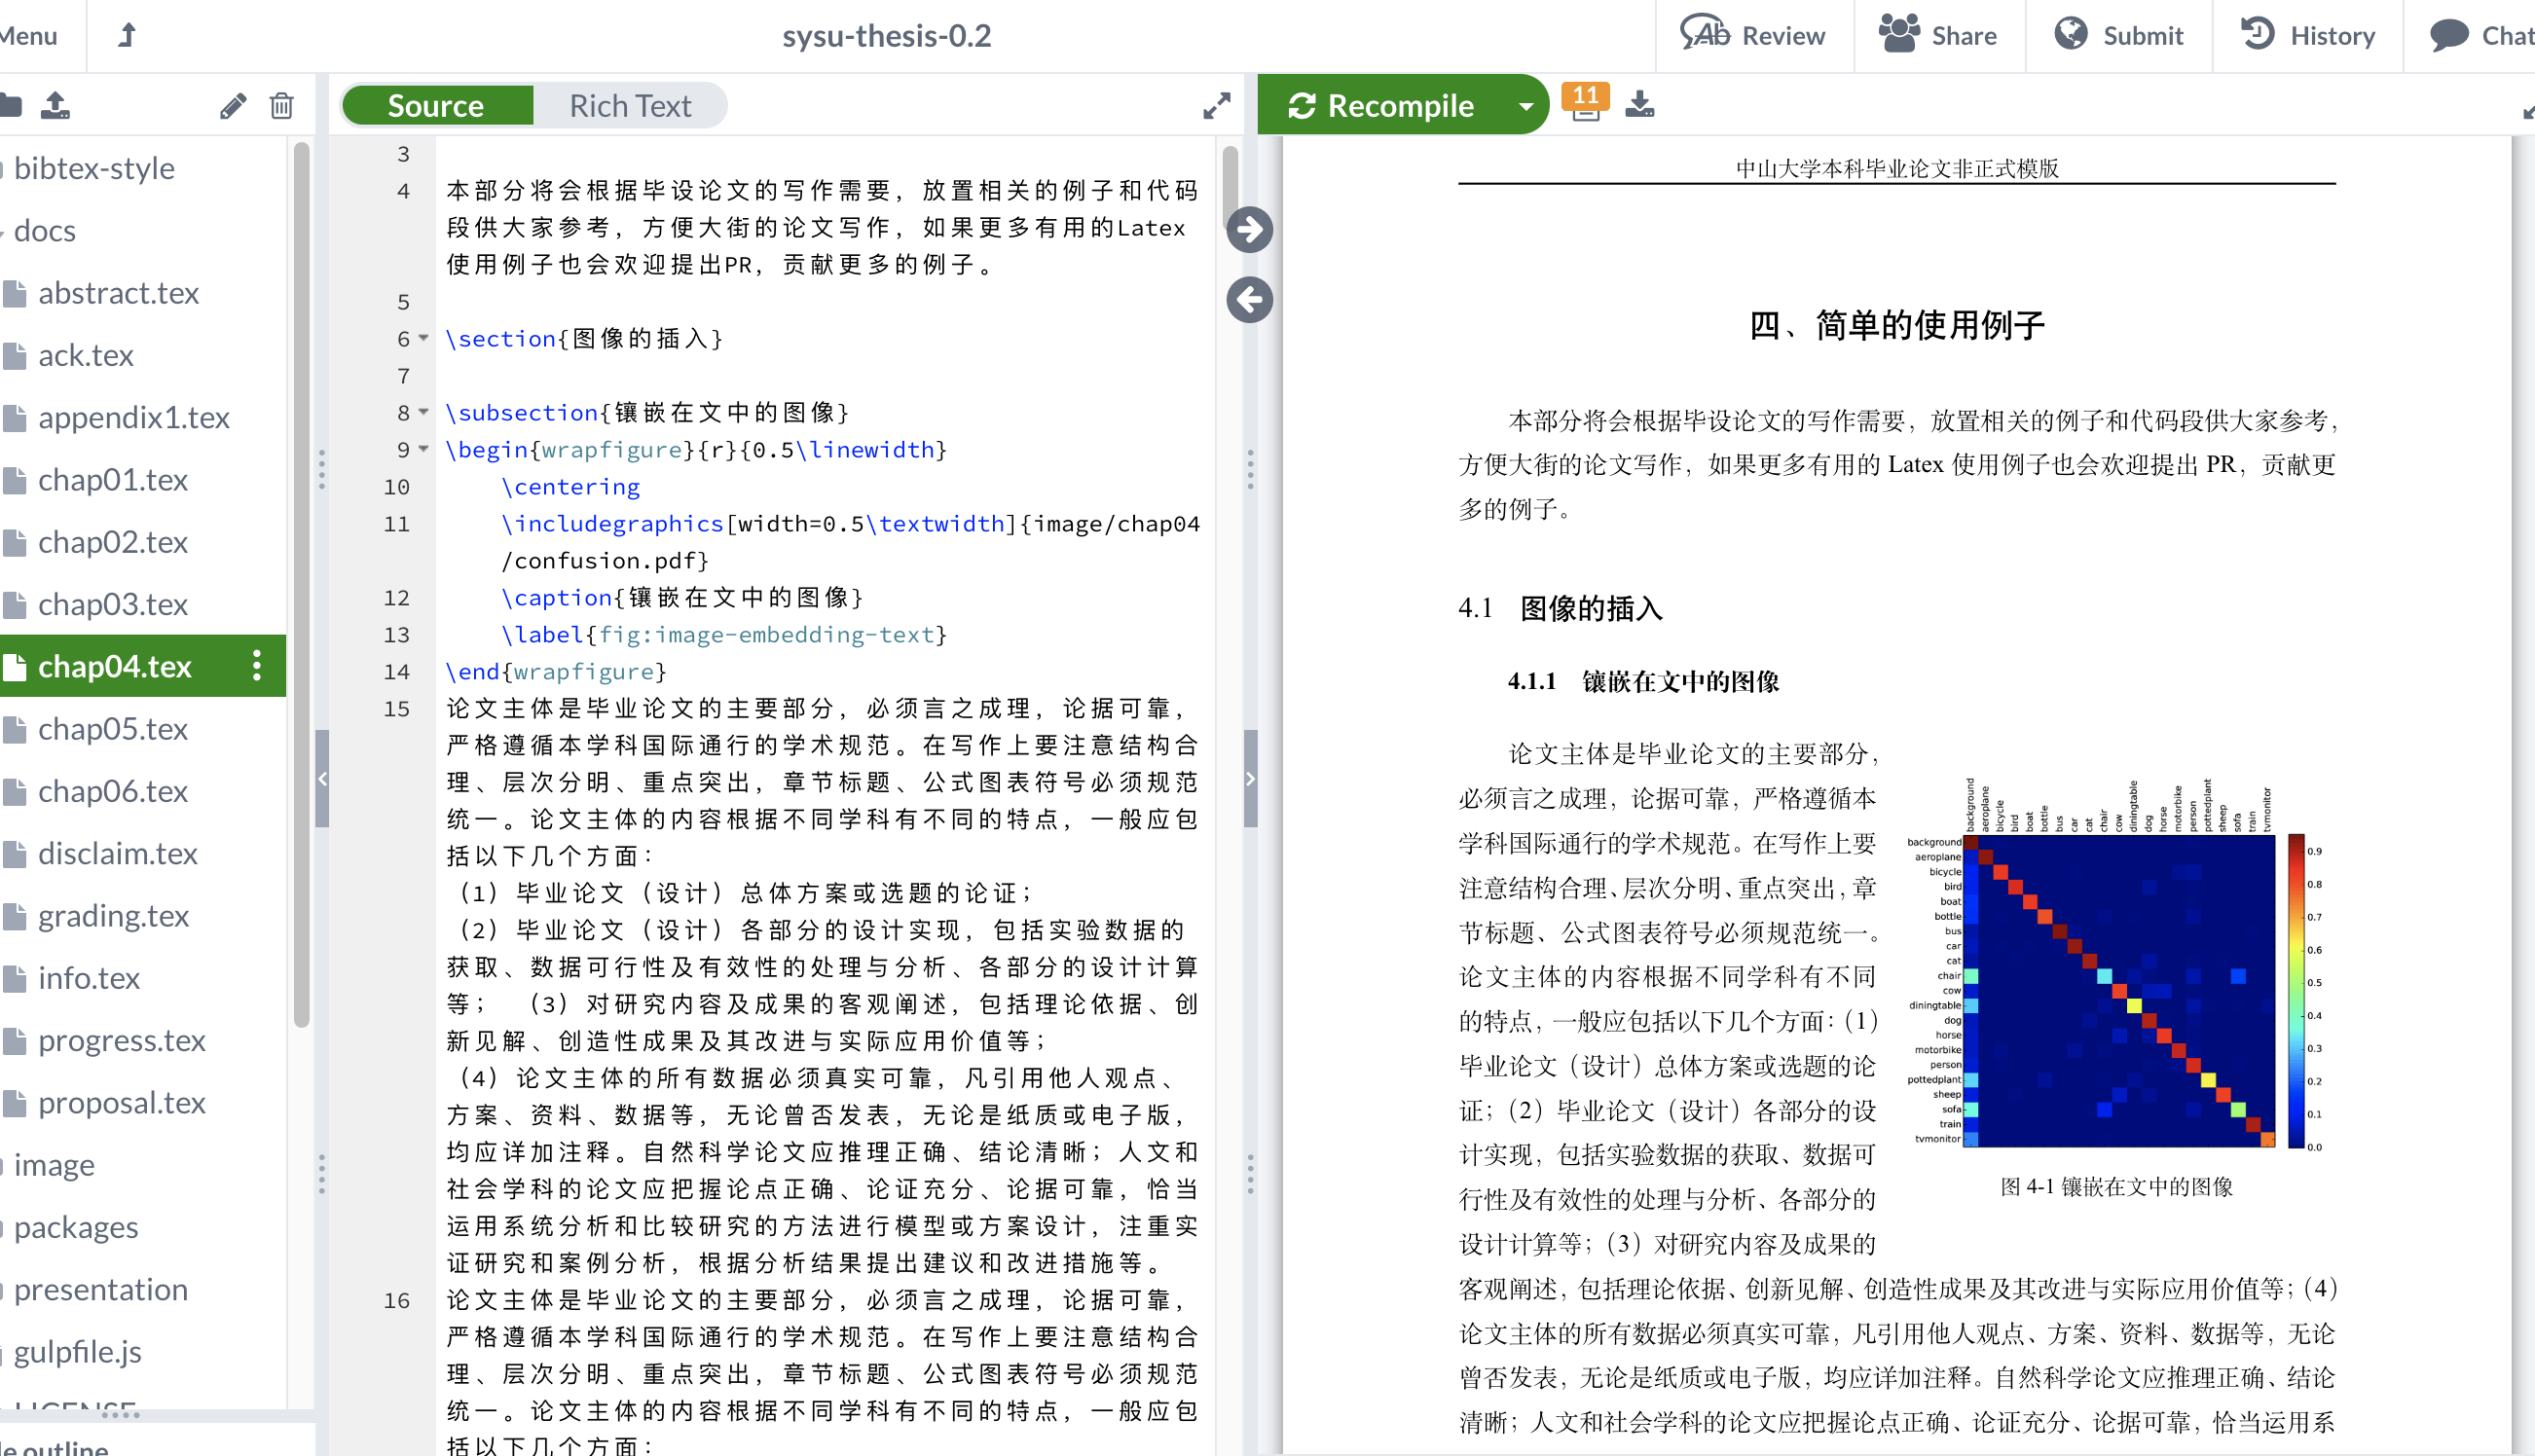
\includegraphics[width=0.9\textwidth]{image/chap03/overleaf-example.jpg}
	\caption{Overleaf使用例子}
	\label{fig:overleaf-example}
\end{figure}



\section{编译环境配置}

编译环境配置相对来说比较简单,下载Tex Live2020并如同一般的程序一样安装即可。

\subsection{编译环境配置:Window篇}

在\url{https://mirrors.tuna.tsinghua.edu.cn/CTAN/systems/texlive/Images/}上下载Tex Live2020并参考教程\footnote{可以参考\url{https://zhuanlan.zhihu.com/p/58811994}}安装即可。

\subsection{编译环境配置:Linux篇}

在\url{https://mirrors.tuna.tsinghua.edu.cn/CTAN/systems/texlive/Images/}上下载Tex Live2020并参考教程\footnote{可以参考\url{https://zhuanlan.zhihu.com/p/55894177}}安装即可。


\subsection{编译环境配置:MacOS篇}

在MacOS上配置Latex的环境,这里我们使用的是MacTex。

\begin{enumerate}
	\item \url{https://www.tug.org/mactex/}下载MacTex安装。
	\item 安装步骤:不详细展开,按照图形界面点击即可, 傻瓜式安装。
\end{enumerate}

TIPS:MacTex文件比较大,有2G多,介意的话可以选择MacTex\_Basic包,只有100M以内,但是如果安装MacTex\_Basic,后期可能会遇到各种缺包的问题。


安装完成之后,可以简单测试一下安装是否成功。如可以查看Texshop应用是否安装好,或者在命令行测试一下\texttt{xelatex}命令是否可用。

\section{写作环境配置}

不同的写作工具对应不同的写作环境。这里我们给出几个工具的配置例子以供参考。

\subsection{模板编译流程}

由于\LaTeX 的限制,本模板需要经过四次编译才能生成完整的论文:

\begin{enumerate}
	\item 先使用xelatex编译一次
	\item 再使用bibtex编译一次
	\item 然后使用xelatex编译两次
\end{enumerate}

本编译流程已经写在Makefile中,修改模板源码后只需要执行\texttt{make pdf}即可按照该流程进行编译并生成最终的pdf。



\subsection{写作环境配置:Visual Studio Code}

Visual Studio Code是微软公司推出的轻量代码编辑器,我们可以做一些简单的配置,便可以用该编辑器修改我们的\LaTeX 模板,并实现一键编译。

\begin{enumerate}
	\item 安装 Visual Studio Code。
	\item 安装 LaTeX Workshop 插件。
\end{enumerate}

本项目的\texttt{.vscode/setting.json}下已经包含了与前面所述编译流程相同的配置。正常配置下,每次修改模板源码后按下保存(Ctrl+S),就能够自动进行编译产生pdf。效果图如\autoref{fig:vscode-example}所示。


\begin{figure}[h]
	\centering
	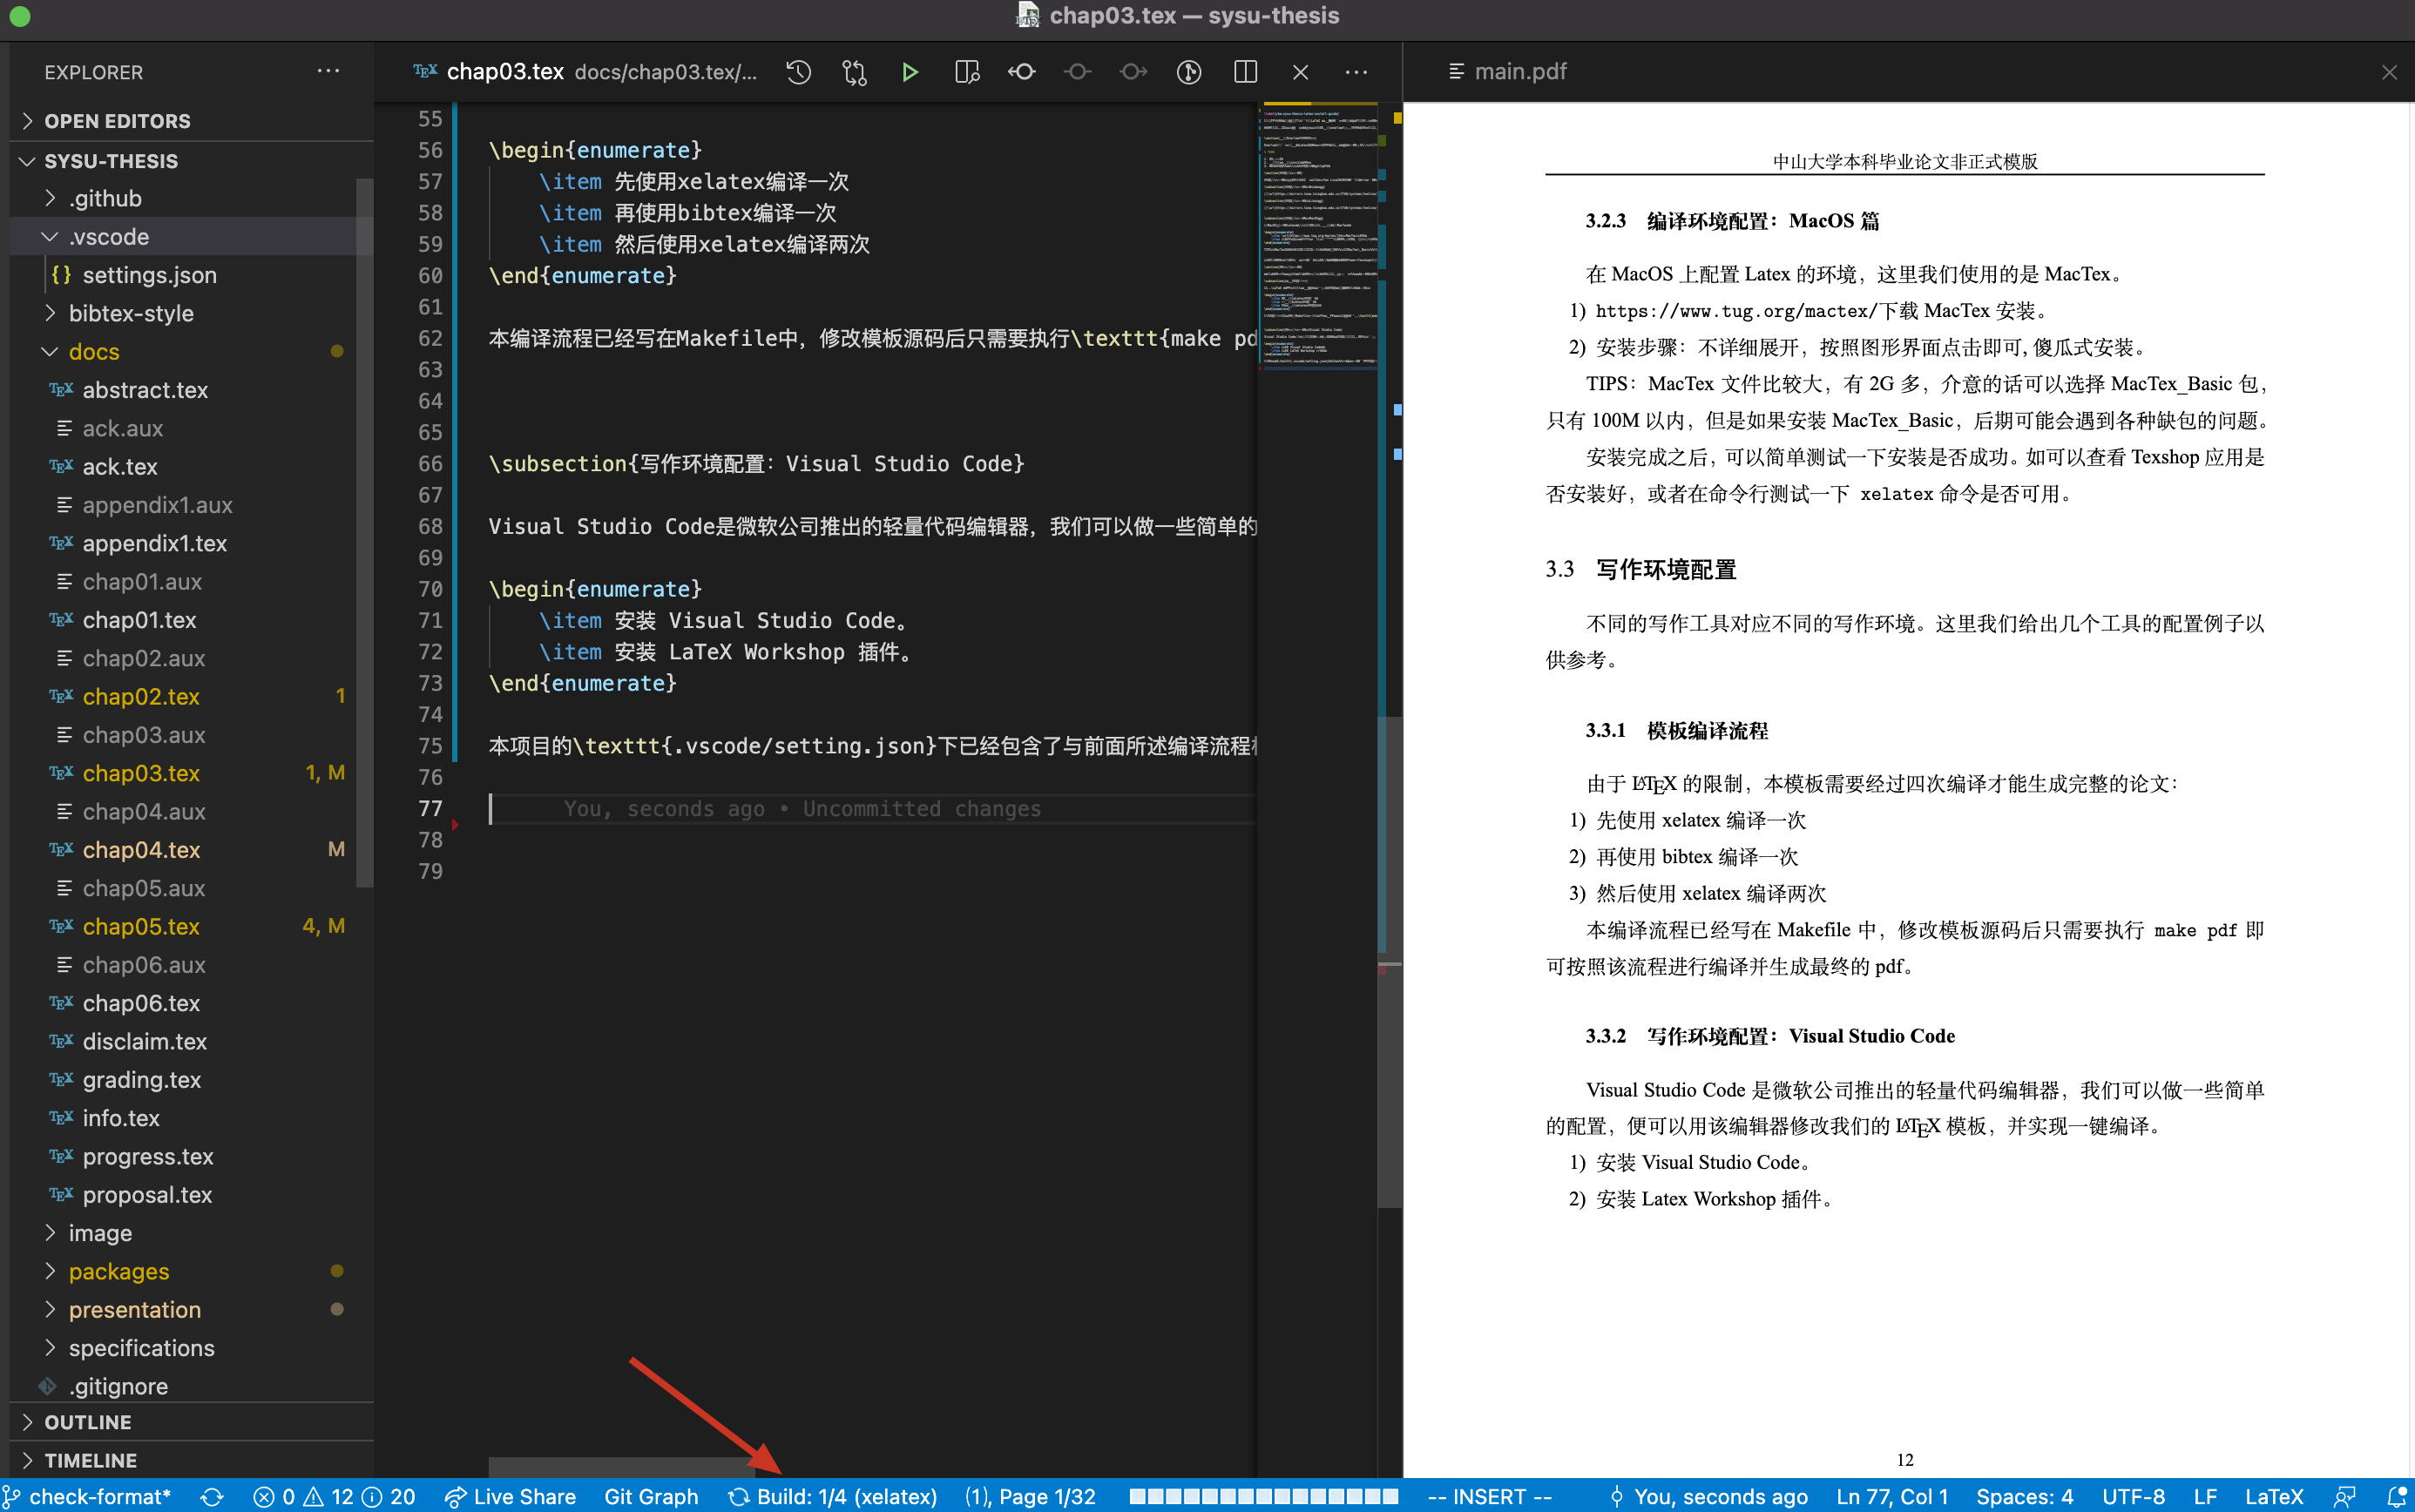
\includegraphics[width=\linewidth]{image/chap03/vscode-example.png}
	\caption{vscode配置好后的样例}
	\label{fig:vscode-example}
\end{figure}


\section{如何开始写毕业论文(设计)}

首先将所有个人信息,包括学号、姓名、专业、论文题目等,在\texttt{./docs/info.tex}中逐项进行更新。

然后我们再编辑\texttt{./docs/abstract.tex}补充论文摘要。

到了论文主体部分,我们可以自行编辑\texttt{./docs/chap01.tex},\texttt{./docs/chap02.tex}等文件进行编辑。如果章数不够,可以自行修改\texttt{main.tex}增加新的章节。

当论文主体编写完成后,我们再编辑\texttt{./docs/ack.tex}作为论文致谢。


% 首先将个人信息写到\texttt{./docs/info.tex}中。
\newclearpage
\chapter{实验及分析}
\label{实验及分析}

\section{硬件环境}
\label{硬件环境}

本节将介绍用于移植测试的华为Atlas 800-9000训练服务器和X86+CUDA对照组平台硬件配置。

\subsection{华为Atlas 800-9000训练服务器简介}
\label{华为Atlas800-9000训练服务器简介}

\newcommand{\tabincell}[2]{\begin{tabular}{@{}#1@{}}#2\end{tabular}}

结合产品主页\footnote{\url{https://e.huawei.com/en/products/cloud-computing-dc/atlas/atlas-800-training-9000}}和本地运行 \lstinline{dmidecode} 指令的结果,我们得到\autoref{华为Atlas800-9000主要配置表}。由于是在单机上进行的算力测试,此处省略了网络和存储等无关参数。

\begin{table}[h] %voc table result
    \centering
    \caption{华为Atlas800-9000主要配置表}
    \label{华为Atlas800-9000主要配置表}
    \resizebox{\textwidth}{!}{
        \begin{tabular}{c|c|c|c}
            \toprule
            组件 & 数量             & 型号         & 参数                          \\
            \midrule
            CPU  & 4                & 华为鲲鹏920  & \tabincell{c}{48Cores @2.6GHz \\L1 Cache 6144KB\\L2 Cache 24567KB\\L3 Cache 49152 kB} \\
            \hline
            内存 & \tabincell{c}{24                                                \\(4 Socket$\times$\\6 Channel)} & 镁光 36ASF4G72PZ-2G9E2 & \tabincell{c}{DDR4\\32GB\\2933 MT/s\\1.2V}\\
            \hline
            NPU  & 8                & 华为昇腾910A & \tabincell{c}{架构:达芬奇    \\FP16算力:320 TFLOPS\\HBM: 32GB, 1200GB/s} \\
            \bottomrule
        \end{tabular}}
\end{table}

容易看出,这台华为Atlas 800-9000是一台高性能服务器,有高达192个ARM64 CPU核,内存总容量共计768GB。同时,其上搭载了8块特殊的``NPU''(neural-network processing units,神经网络处理器),已在\autoref{华为昇腾910硬件架构}详细分析。

\subsection{X86+CUDA对照平台简介}

结合结合产品主页\footnote{\url{https://www.nvidia.com/en-us/data-center/a100/}}和本地运行 \lstinline{dmidecode} 指令的结果,我们得到\autoref{X86+CUDA对照组平台主要配置表}。由于是在单机上进行的算力测试,此处省略了网络和存储等无关参数。

\begin{table}[h] %voc table result
    \centering
    \caption{X86+CUDA对照组平台主要配置表}
    \label{X86+CUDA对照组平台主要配置表}
    \resizebox{\textwidth}{!}{
        \begin{tabular}{c|c|c|c}
            \toprule
            组件 & 数量             & 型号                  & 参数                                    \\
            \midrule
            CPU  & 2                & AMD 霄龙 7542         & \tabincell{c}{32Cores, 64Threads@2.9GHz \\L1 Cache 2MB\\L2 Cache 16MB\\L3 Cache 128 MB} \\
            \hline
            内存 & \tabincell{c}{32                                                                   \\(4 Socket$\times$\\8 Channel)} & 海力士 HMAA8GR7AJR4N-XN & \tabincell{c}{DDR4\\64GB\\2933 MT/s\\1.2V}\\
            \hline
            GPU  & 8                & 英伟达 A100-SXM4-40GB & \tabincell{c}{架构:安培                \\FP16算力:312 TFLOPS(TensorCore)\\
                FP32算力:156 TFLOPS(TensorCore)                                                    \\
                HBM: 40GB, 1555GB/s}                                                                  \\
            \bottomrule
        \end{tabular}}
\end{table}

该平台作为对照组的优势是,其拥有与移植平台相近的配置,且搭载的加速卡拥有相同的7nm制程、相近的FP16理论矩阵算力。当然,仍然要指出的是,华为Atlas 800-9000所搭载的鲲鹏920与对照组AMD霄龙7542的架构完全不同,前者是ARM64,后者是X86;并且,前者拥有更多的核心,后者有更高的频率和更大的Cache。

\section{软件环境}

\autoref{测试平台软件环境表}给出了我们的实验环境,表中软件除了针对昇腾异构加速卡特殊优化的hpl-ai@2.3d+ascendcl及其依赖CANN V100R020C10外,均可通过包管理器spack\cite{2015The}与我们的spack软件扩展源一键安装。\footnote{我们使用了spack包管理器管理需要的诸多软件依赖,其优势在于提供了一套易用的源码安装管理。我们也将我们的HPL-AI发布在\url{https://github.com/SYSU-SCC/sysu-scc-spack-repo}中,这使得其可以很容易地在其他环境中被部署、复现。}

\begin{table}[h]
    \centering
    \caption{测试平台软件环境表}
    \label{测试平台软件环境表}
    \resizebox{\textwidth}{!}{

        \begin{tabular}{c|c|c}
            \toprule

            平台     & 华为Atlas 800-9000                            & X86+CUDA对照组平台        \\

            \midrule

            操作系统 & linux-centos7-aarch64                         & linux-debian9-zen2        \\

            \hline

            驱动版本 & ascend-dmi 20.1.rc1                           & NVIDIA-SMI 450.80.02      \\

            \hline

            特定软件 & \begin{tabular}[c]{@{}c@{}}
                CANN V100R020C10 \\
                hpl-ai@2.3d\%gcc@7.5.0+ascendcl
            \end{tabular}                     & \begin{tabular}[c]{@{}c@{}}
                cuda@11.0.2\%gcc@7.5.0            \\
                blaspp@2021.04.01\%gcc@7.5.0+cuda \\
                hpl-ai@2.3d+cuda                  \\
                hpl-ai@2.3d+cuda $\backslash$     \\
                cublasGemmEx\_computeType=fp16
            \end{tabular} \\

            \hline

            通用软件 & \multicolumn{2}{c}{\begin{tabular}[c]{@{}c@{}}
                    spack 0.16.1                              \\
                    gcc@7.5.0                                 \\
                    openmpi@3.1.6\%gcc@7.5.0                  \\
                    openblas@0.3.13\%gcc@7.5.0 threads=openmp \\
                    hpl@2.3\%gcc@7.5.0                        \\
                    blaspp@2021.04.01\%gcc@7.5.0              \\
                    hpl-ai@2.3d\%gcc@7.5.0                    \\
                \end{tabular}}                             \\

            \bottomrule
        \end{tabular}}
\end{table}

\subsection{对比软件介绍}

\autoref{对比软件介绍表}列出了我们实现的HPL-AI软件包的和用于对照组的开源HPL软件包。

\begin{table}[h] %voc table result
    \centering
    \caption{对比软件介绍表}
    \label{对比软件介绍表}
    \resizebox{\textwidth}{!}{
        \begin{tabular}{c|c|c}
            \toprule
            软件                 & 运行设备 & 介绍                             \\
            \midrule
            hpl@2.3              & CPU      & \tabincell{c}{HPL标准实现。      \\用于对照组。}\\
            \hline
            hpl-ai@2.3d          & CPU      & \tabincell{c}{我们的HPL-AI实现。 \\在LU分解阶段使用单精度。}\\
            \hline
            hpl-ai@2.3d+ascendcl & CPU+NPU  & \tabincell{c}{
                我们的HPL-AI实现。                                             \\
                在LU分解阶段使用单精度。                                       \\
                GEMM阶段会在NPU上将FP32格式的矩阵继续压缩成FP16格式,          \\
                然后调用MatMulV2。}                                            \\
            \hline
            \tabincell{c}{
            hpl-ai@2.3d+cuda}    & CPU+GPU  & \tabincell{c}{
                我们的HPL-AI实现。                                             \\
                在LU分解阶段使用单精度。                                       \\
                使用GPU完成gemm和trsm过程。}                                   \\
            \hline
            \tabincell{c}{
                hpl-ai@2.3d+cuda $\backslash$                                  \\
                cublasGemmEx\_computeType=fp16
            }                    & CPU+GPU  & \tabincell{c}{
                我们的HPL-AI实现。                                             \\
                在LU分解阶段使用单精度。                                       \\
                gemm阶段会在GPU上调用cublasGemmEx,                            \\
                将FP32格式的矩阵继续压缩成FP16格式并进行矩阵乘法。}            \\
            \bottomrule
        \end{tabular}}
\end{table}

\subsection{软件依赖}
\label{软件依赖}

CPU厂商通常会针对自己的硬件发布经过调优的BLAS实现,如Intel的mkl库、AMD的amdblis库等(这些厂商甚至会发布针对自己硬件优化的Linpack实现,如Intel的mp\_linpack、NVIDIA的hpc-benchmark),但这为我们在不同平台上进行性能比较带来了不便。一方面,这些调优后的数学库大部分情况下都不能移植到其他平台(或是性能表现很差),难以控制实验中的变量;另一方面,其实现通常不开源,这使得我们更难分析运行时的瓶颈是来自于算法本身还是调用的BLAS。为此,我们在测试时使用openblas@0.3.13\footnote{需要注意的是,spack 0.16.1内建的openblas@0.3.5存在问题,详见\autoref{运行策略}。我们在自己的spack软件扩展源提供了修复该错误的openblas@0.3.13及改变软件依赖的blaspp安装脚本。},该库提供了X86、ARM、RISC-V等多种CPU平台的开源实现。

同理,我们选择了openmpi@3.1.6作为作为统一的MPI依赖,并且所有提供源码的软件包统一使用gcc@7.5.0从源码编译。

\subsection{MPI进程及绑核设置}

\autoref{硬件环境}中提到,不管是华为Atlas 800-9000还是用于对照的X86+CUDA平台,都有八张加速卡。我们让单张加速卡对应一个单独进程,因此如果没有特别提及的情况下统一使用八个MPI进程。同时,使用openmpi@3.1.6默认的绑核设置。

此外,由于下述实验都是在单机上进行的,因此不涉及MPI通信协议的选择。

\subsection{OpenMP线程数设置}

即使是GPU/NPU上运行的HPL-AI,都有相当一部分计算量(主要是level-1和level-2的BLAS调用)是放在CPU上的,因此需要设置openblas库运行时用于单进程的线程数量。设置的原则是充分使用CPU的每个计算核心。对于Atlas,我们设置8个进程每个进程24线程;对于X86+CUDA对照平台,我们设置8个进程每个进程16线程。

\subsection{HPL.dat}

运行参数的设置是一个稍微复杂一些的问题。一方面,作为benchmark,它需要尽量契合硬件配置,以充分利用机器能提供的最高算力;另一方面,在对照实验中,我们应当控制变量,从而尽可能排除由于参数设置不同影响实验结果的情况。因此,有必要使用一个尽可能通用的运行参数设置,同时针对各个实验进行微调。如果没有特别提及的输入参数,均默认使用\autoref{HPL.dat}中的内容。

\begin{figure}[h]
    \centering
    \begin{bash}
        HPLinpack and HPL-AI benchmark input file
        National Supercomputer Center in Guangzhou, Sun Yat-sen University
        HPL.out      output file name (if any)
        6            device out (6=stdout,7=stderr,file)
        1            # of problems sizes (N)
        131072       Ns
        2            # of NBs
        192 192      NBs
        0            PMAP process mapping (0=Row-,1=Column-major)
        1            # of process grids (P x Q)
        2            Ps
        4            Qs
        16.0         threshold
        1            # of panel fact
        2 1 0        PFACTs (0=left, 1=Crout, 2=Right)
        1            # of recursive stopping criterium
        2 8          NBMINs (>= 1)
        1            # of panels in recursion
        2            NDIVs
        1            # of recursive panel fact.
        2 1 0        RFACTs (0=left, 1=Crout, 2=Right)
        1            # of broadcast
        0 2          BCASTs (0=1rg,1=1rM,2=2rg,3=2rM,4=Lng,5=LnM)
        1            # of lookahead depth
        1            DEPTHs (>=0)
        1            SWAP (0=bin-exch,1=long,2=mix)
        192          swapping threshold
        1            L1 in (0=transposed,1=no-transposed) form
        0            U  in (0=transposed,1=no-transposed) form
        1            Equilibration (0=no,1=yes)
        16           memory alignment in HPLAI_T_AFLOAT (> 0)
    \end{bash}
    \caption{HPL.dat}
    \label{HPL.dat}
\end{figure}

此处重复设置$\mathit{NB}$以使用\autoref{热身运行}中的策略。值得注意的是,此处设置$\mathit{NB}=192$,这是适合于CPU的参数,以减少Cache Miss。在异构处理器上运行HPL或HPL-AI时通常需要取更大的值,从而充分利用异构处理器的矩阵算力。在本文中对于NPU我们选取$\mathit{NB}=4096$,对于GPU我们选取$\mathit{NB}=2048$。

\section{实验与分析}

我们设计了如下三个实验,对我们的HPL-AI软件包进行测试。

\subsection{AscendCL接口与算子调用实验}
\label{AscendCL接口与算子调用实验}

运行我们的Profile代码\footnote{我们的完整Profile代码提供在\url{https://wu-kan.cn/2021/03/21/\%E5\%8D\%8E\%E4\%B8\%BA\%E6\%98\%87\%E8\%85\%BE910\%E4\%BD\%BF\%E7\%94\%A8\%E5\%88\%9D\%E6\%8E\%A2/}}得到\autoref{AscendCL接口/算子耗时表},给出$\left(M,N,K\right)=\left(8192,8192,8192\right)$时各接口和算子的耗时情况。

\begin{table}[h] %voc table result
    \centering
    \caption{AscendCL接口/算子耗时表}
    \label{AscendCL接口/算子耗时表}
    \begin{tabular}{c|c|c}
        \toprule
        接口/算子              & 运行时间    & 有效算力       \\
        \midrule
        aclInit                & 4.422 ms    & /              \\
        \hline
        aclrtCreateContext     & 351.026 ms  & /              \\
        \hline
        aclrtSetCurrentContext & 0.006 ms    & /              \\
        \hline
        aclrtMalloc            & 198.336 ms  & /              \\
        \hline
        aclrtMemcpyAsync       & 11.689 ms   & /              \\
        \hline
        Cast(aclFloat16)       & 0.498 ms    & /              \\
        \hline
        Cast(float)            & 0.484 ms    & /              \\
        \hline
        MatMulV2(FP16)         & 5.613 ms    & 195.887 TFLOPS \\
        \hline
        MatMulV2(FP32)         & 1154.355 ms & 0.952 TFLOPS   \\
        \hline
        MatMul(FP16)           & 5.610 ms    & 195.991 TFLOPS \\
        \hline
        MatMul(FP32)           & 1154.473 ms & 0.952 TFLOPS   \\
        \hline
        GEMM(FP16)             & 202.152 ms  & 5.439 TFLOPS   \\
        \hline
        aclrtFree              & 59.107 ms   & /              \\
        \hline
        aclrtDestroyContext    & 186.624 ms  & /              \\
        \hline
        aclFinalize            & 349.656 ms  & /              \\
        \hline
        \bottomrule
    \end{tabular}
\end{table}

根据 Profile 结果可以得到以下结论:

\begin{itemize}
    \item 创建上下文、申请内存、释放内存、释放上下文、去初始化的开销都很大,需要在运行算法时尽量避免相关调用。
    \item \lstinline{MatMul} 算子调用时间远低于三次 \lstinline{aclrtMemcpy}(表中Memcpy仅包含一个矩阵拷贝的时间)。换言之,开销主要在主机和设备的通信,而非设备上的计算上。
    \item 切换上下文开销很低,但创建释放上下文的开销仍然很高,必要时仍要使用 \lstinline{aclrtStream}。
    \item \lstinline{GEMM} 算子性能远低于 \lstinline{MatMul} 和 \lstinline{MatMulV2},合理推断向量单元和标量单元性能远低于矩阵单元。
    \item 使用单精度的MatMul比半精度的MatMul慢了几个数量级,比较鸡肋。
\end{itemize}

\subsection{可扩展性验证实验}

对于$N\in\lbrace 4096,8192,16384,32768,65536,131072\rbrace$,在Atlas上使用8、16、32、64、128、192核心运行hpl-ai@2.3d,得到\autoref{HPL-AI效率测试表}(/TFLOPS),验证HPL-AI软件包的可扩展性。

\begin{table}[h] %voc table result
    \centering
    \caption{HPL-AI效率测试表}
    \label{HPL-AI效率测试表}
    \begin{tabular}{c|cccccc}
        \toprule
        问题规模$\backslash$并行核数 & 8     & 16    & 32    & 64    & 128   & 192   \\
        \midrule
        4096                         & 0.013 & 0.215 & 0.323 & 0.428 & 0.456 & 0.112 \\
        \hline
        8192                         & 0.016 & 0.305 & 0.526 & 0.816 & 1.052 & 1.080 \\
        \hline
        16384                        & 0.019 & 0.358 & 0.673 & 1.172 & 1.683 & 2.018 \\
        \hline
        32768                        & 0.020 & 0.389 & 0.752 & 1.331 & 2.331 & 2.766 \\
        \hline
        65536                        & 0.021 & 0.417 & 0.816 & 1.532 & 2.732 & 3.660 \\
        \hline
        131072                       & 0.022 & 0.432 & 0.853 & 1.660 & 3.103 & 4.340 \\
        \bottomrule
    \end{tabular}
\end{table}

由\autoref{HPL-AI具有强可扩展性}可以看到,问题规模足够大时,固定问题(不妨取$N=131072$)规模,有效算力随并行核数增加线性增长,该应用有\textbf{强可扩展性}。在问题规模小的时候(如$N=4096$),单节点过多的并行核数反而会导致诸如伪共享\footnote{\url{https://en.wikipedia.org/wiki/False_sharing}}的问题,使程序变慢。

\begin{figure}[h]
    \centering
    \begin{tikzpicture}
        \begin{axis}[xlabel=并行核数,ylabel=效率/TFLOPS,legend pos=outer north east] % 将图例放在图外,位于图的东北角
            \addplot
            coordinates                             % 绘制原始数据的折线图
                {           		                % X,Y的原始数据
                    (8,0.22)
                    (16,0.432)
                    (32,0.853)
                    (64,1.660)
                    (128,3.103)
                    (192,4.340)
                };
            \addlegendentry{$N=131072$}
            \addplot
            coordinates                              % 绘制原始数据的折线图
                {           		                % X,Y的原始数据
                    (8,0.21)
                    (16,0.417)
                    (32,0.816)
                    (64,1.532)
                    (128,2.732)
                    (192,3.660)
                };
            \addlegendentry{$N=65536$}
            \addplot
            coordinates                                 % 绘制原始数据的折线图
                {           		                % X,Y的原始数据
                    (8,0.020)
                    (16,0.389)
                    (32,0.752)
                    (64,1.331)
                    (128,2.331)
                    (192,2.766)
                };
            \addlegendentry{$N=32768$}
            \addplot
            coordinates                                 % 绘制原始数据的折线图
                {           		                % X,Y的原始数据
                    (8,0.019)
                    (16,0.358)
                    (32,0.673)
                    (64,1.172)
                    (128,1.683)
                    (192,2.018)
                };
            \addlegendentry{$N=16384$}
            \addplot
            coordinates                                 % 绘制原始数据的折线图
                {           		                % X,Y的原始数据
                    (8,0.016)
                    (16,0.305)
                    (32,0.526)
                    (64,0.816)
                    (128,1.052)
                    (192,1.080)
                };
            \addlegendentry{$N=8192$}
            \addplot
            coordinates                               % 绘制原始数据的折线图
                {           		                % X,Y的原始数据
                    (8,0.013)
                    (16,0.215)
                    (32,0.323)
                    (64,0.428)
                    (128,0.456)
                    (192,0.112)
                };
            \addlegendentry{$N=4096$}
        \end{axis}
    \end{tikzpicture}
    \caption{HPL-AI具有强可扩展性}
    \label{HPL-AI具有强可扩展性}
\end{figure}

\subsection{NPU加速验证实验}

在Atlas上运行hpl@2.3、hpl-ai@2.3d、hpl-ai@2.3d+ascendcl($\mathit{NB}=4096$),在X86+CUDA验证平台运行hpl@2.3、hpl-ai@2.3d、hpl-ai@2.3d+cuda($\mathit{NB}=2048$)、hpl-ai@2.3d+cuda cublasGemmEx\_computeType=fp16($\mathit{NB}=2048$),对比并验证hpl-ai@2.3d+ascendcl的移植加速效果,得到\autoref{NPU加速验证表}和\autoref{实测性能对照图}。

\begin{table}[h] %voc table result
    \centering
    \caption{NPU加速验证表}
    \label{NPU加速验证表}
    \resizebox{\textwidth}{!}{
        \begin{tabular}{c|c|c|c|c}
            \toprule
            编号                  & 测试软件包                                      & 测试平台 & 运行时间      & 有效算力     \\
            \midrule
            \#1                   & hpl@2.3                                         & Atlas    & 905.95s       & 1.657 TFLOPS \\
            \hline
            \#2                   & hpl-ai@2.3d                                     & Atlas    & 345.90s       & 4.340 TFLOPS \\
            \hline
            \#3                   & \tabincell{c}{hpl-ai@2.3d+ascendcl $\backslash$                                           \\($\mathit{NB}=4096$)} & Atlas & 261.84s & 5.733 TFLOPS  \\
            \hline
            \#4                   & hpl@2.3                                         & X86+CUDA & 718.88s       & 2.088 TFLOPS \\
            \hline
            \#5                   & hpl-ai@2.3d                                     & X86+CUDA & 360.70s       & 4.162 TFLOPS \\
            \hline
            \#6                   & \tabincell{c}{
                hpl-ai@2.3d+cuda $\backslash$                                                                                 \\
            ($\mathit{NB}=2048$)} & X86+CUDA                                        & 112.95s  & 13.291 TFLOPS                \\
            \hline
            \#7                   & \tabincell{c}{
                hpl-ai@2.3d+cuda $\backslash$                                                                                 \\
                cublasGemmEx\_computeType=fp16 $\backslash$                                                                   \\($\mathit{NB}=2048$)} & X86+CUDA & 103.69s & 14.477 TFLOPS  \\
            \bottomrule
        \end{tabular}}

\end{table}

\begin{figure}[h]
    \centering
    \begin{tikzpicture}
        \begin{axis}
            [
                ybar,
                ylabel={实测性能/TFLOPS}, % the ylabel must precede a # symbol.
                xlabel={实验算例},
                symbolic x coords={\#1, \#2, \#3, \#4, \#5, \#6, \#7},
                legend pos=outer north east
            ]

            \addplot coordinates {(\#1, 1.657) (\#2, 4.296) (\#3, 5.733)};
            \addlegendentry{ARM+NPU};
            \addplot coordinates {(\#4, 2.088) (\#5, 4.162) (\#6, 13.291) (\#7, 14.477)};
            \addlegendentry{X86+GPU};

        \end{axis}
    \end{tikzpicture}
    \caption{实测性能对照图}
    \label{实测性能对照图}
\end{figure}

对比\#1、\#2可知,相对于HPL,我们的HPL-AI在Atlas使用单精度取得了$2.59\times$的加速比。一方面,使用单精度运算可以使用比FP64运算单元更多的FP32计算单元;另一方面,使用低精度计算也减少了算法运行时的通信开销和CacheMiss。

对比\#5、\#6、\#7可知,我们的HPL-AI可以使用异构加速卡取得明显性能提升,且引入混合精度的计算可以获得更高的收益。

对比\#3、\#7,虽然此处的参数$N$设置虽然均远没有让两台机器的异构处理器满载\footnote{此处选择的$N$需要大量不同规格的Cast+MatMulV2算子,即使使用\autoref{算子编译脚本}中的并行编译脚本也需要数个小时才能进行一次完整测试。继续扩大$N$会导致算子数量的进一步上升,短时间内很难进行进行参数调优。},也可明显对比NPU与GPU的性能差异。

一方面,由\autoref{AscendCL接口与算子调用实验}可知,在我们的应用中使用昇腾910的瓶颈主要来自于三次\lstinline{aclrtMemcpy}过程,其耗时是调用\lstinline{MatMul}算子的六倍之多;而此处我们使用的A100是NVLink接口版本,其带宽高达600GB/S,远大于使用昇腾910的64GB/S(PCIe4.0)\footnote{\autoref{AscendCL接口与算子调用实验}中实测性能约为21GB/S},因此可以更加充分的利用异构加速卡上的算力。因此,通信带宽是昇腾910的一个明显瓶颈;若后续版本的昇腾处理器提升其与主机的通信带宽,则可在HPL-AI基准中获得更高的计算效率。

另一方面,昇腾910是专门面向为AI应用设计的处理器,本身并非适合通用计算,而NVIDIA A100则可以使用cuBLAS中专门调优过的gemm接口和trsm接口。国产异构处理器在软件生态建设上仍任重而道远。

\newclearpage
\chapter{总结与展望}
\label{总结与展望}

\section{总结}

在本文中,我们首先介绍了HPL-AI基准的背景和相关工作,并分析了HPL-AI的基本规则,介绍了使用到的矩阵生成算法、LU分解算法、数值迭代算法。

随后,基于对硬件架构的分析以及对接口、算子调用的Profiling,我们面向华为Atlas 800-9000 AI训练服务器上搭载的国产异构处理器昇腾910设计出一套合理的移植优化方案,以充分利用其半精度算力。

然后,我们以X86+CUDA平台为对照组,将HPL和我们的HPL-AI性能进行对比。实验结果表明,借助混合精度矩阵分解算法和数值迭代算法,我们的实现能获得与HPL相当的计算精度,且得到明显性能提升。

我们的工作为不同平台上的HPL-AI基准测试给出可信参照,也对在昇腾平台或其他异构计算平台上的HPC/AI应用优化有很强的指导意义。

\section{展望}

时间所限,在本次毕业设计前我仅完成了对HPL-AI的初步实现和移植。后续交付鹏城实验室后,以下工作仍然是值得被考虑的:

\begin{enumerate}
    \item 使用昇腾910的RC模式\footnote{\url{https://support.huaweicloud.com/asdevg-c-cann/atlassample_14_0010.html}}启动HPL-AI,免去通信开销。由于其板载CPU性能远低于主机端CPU性能,且内存只有16GB,实际表现仍是值得商榷的。
    \item 可以参照英伟达 hpl-2.0\_FERMI\_v15.tgz \footnote{\url{https://developer.nvidia.com/rdp/assets/cuda-accelerated-linpack-linux64}}中的手段,使用多流等手段提高异构处理器的负载;
    \item 由于CPU同为ARM架构,\cite{DBLP:conf/scala-ws/KudoNII20}在``富岳''上的工作对我们有很强的参考意义。例如:
          \begin{enumerate}
              \item Single iteration scheme for IR相较于GMRES开销更低;
              \item On-The-Fly matrix generation可减少主机端内存上的占用。当然,对于我们的移植平台,限制可能更多来自于异构处理器的存储空间。
          \end{enumerate}
    \item 探索传统HPL的优化方法,如针对``鹏城云脑II''的网络拓扑,优化HPL-AI的MPI调用。由于我们的HPL-AI是参照HPL实现的,大部分对于HPL的优化都可以考虑应用到HPL-AI上。
\end{enumerate}

\newclearpage

% 结语

% 附录部分
\backmatter
% 参考文献. 因不需要纳入章节目录, 故放入附录部分
% 实际上参考文献是属于论文主体部分
\makereferences

% 附录
{
    \appendix
    \chapter{补充更多细节}

\section{补充图}

\subsection{补充图}

这是附录内容,应该用宋体小四号字体。

\begin{figure}[h!]
	\centering
	\makebox[0.16\textwidth]{\scriptsize 图像}
	\makebox[0.16\textwidth]{\scriptsize 真值}
	\makebox[0.16\textwidth]{\scriptsize Grid-5LSTM1}
	\makebox[0.16\textwidth]{\scriptsize Grid-5LSTM3}
	\makebox[0.16\textwidth]{\scriptsize Grid-5LSTM5} \\
	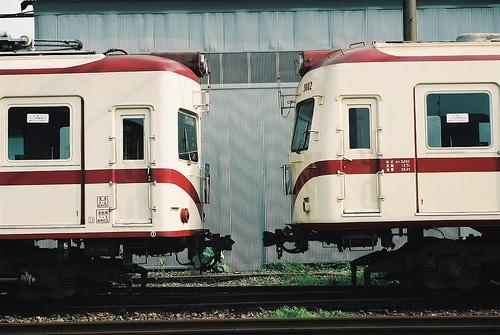
\includegraphics[width=0.16\textwidth]{image/appendix1/2007_000042.jpg}
	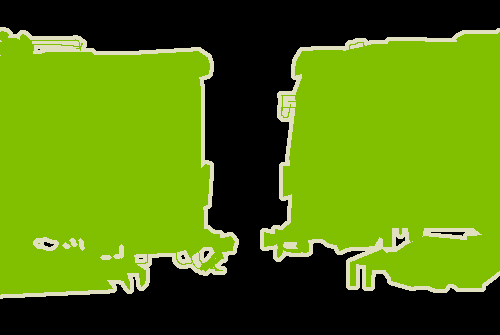
\includegraphics[width=0.16\textwidth]{image/appendix1/2007_000042.png}
	
\includegraphics[width=0.16\textwidth]{image/appendix1/1/2007_000042.png}
	
\includegraphics[width=0.16\textwidth]{image/appendix1/3/2007_000042.png}
	
\includegraphics[width=0.16\textwidth]{image/appendix1/5/2007_000042.png} \\

	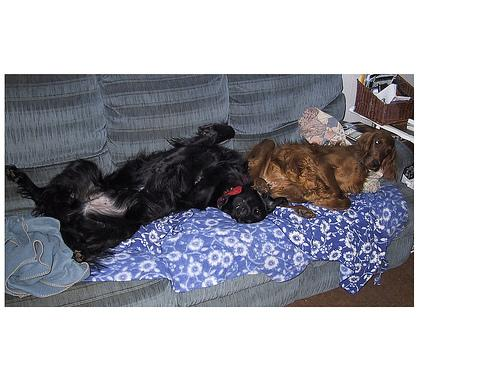
\includegraphics[width=0.16\textwidth]{image/appendix1/2011_003256.jpg}
	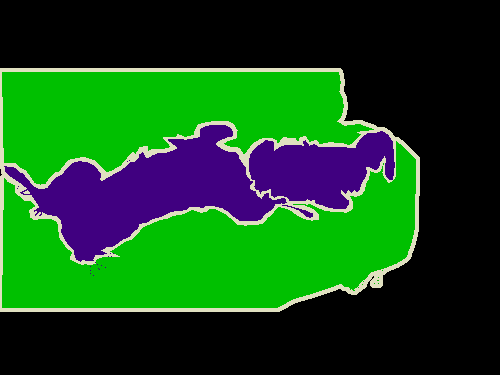
\includegraphics[width=0.16\textwidth]{image/appendix1/2011_003256.png}
	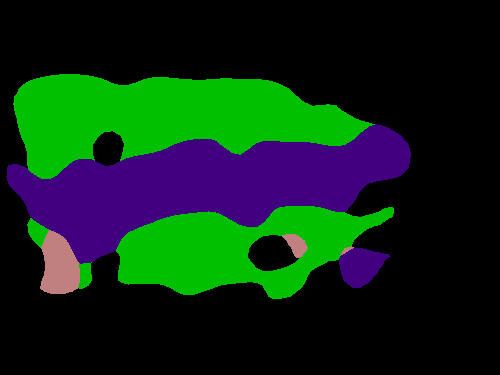
\includegraphics[width=0.16\textwidth]{image/appendix1/1/2011_003256.png}
	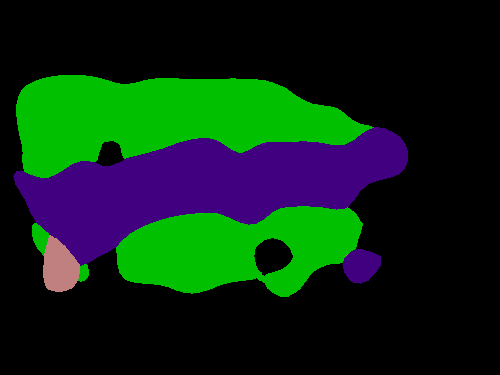
\includegraphics[width=0.16\textwidth]{image/appendix1/3/2011_003256.png}
	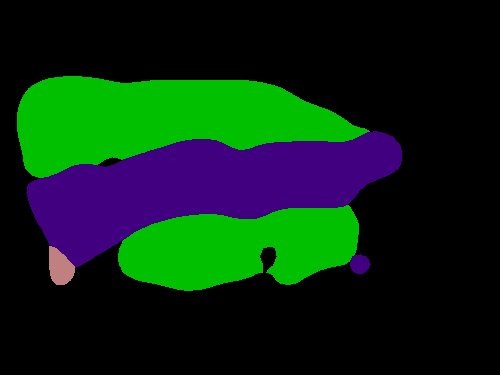
\includegraphics[width=0.16\textwidth]{image/appendix1/5/2011_003256.png} \\
	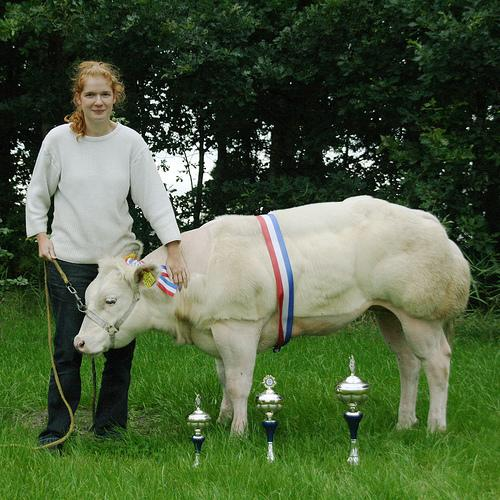
\includegraphics[width=0.16\textwidth]{image/appendix1/2011_001159.jpg}
	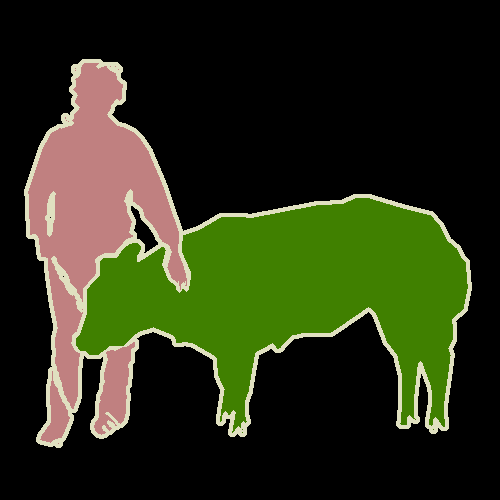
\includegraphics[width=0.16\textwidth]{image/appendix1/2011_001159.png}
	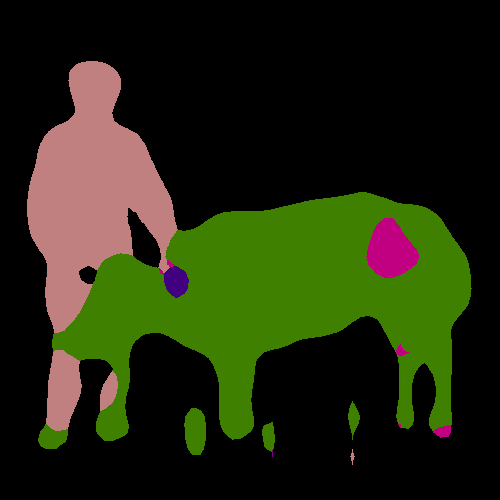
\includegraphics[width=0.16\textwidth]{image/appendix1/1/2011_001159.png}
	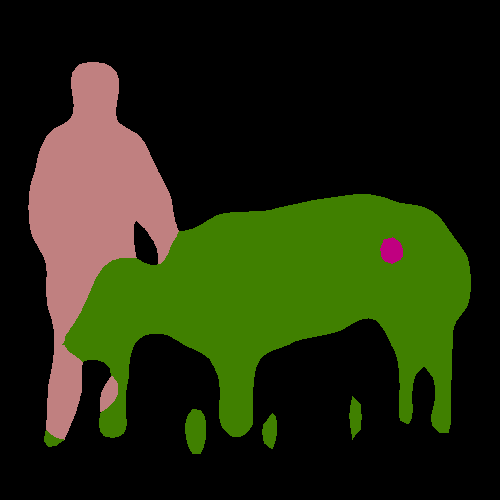
\includegraphics[width=0.16\textwidth]{image/appendix1/3/2011_001159.png}
	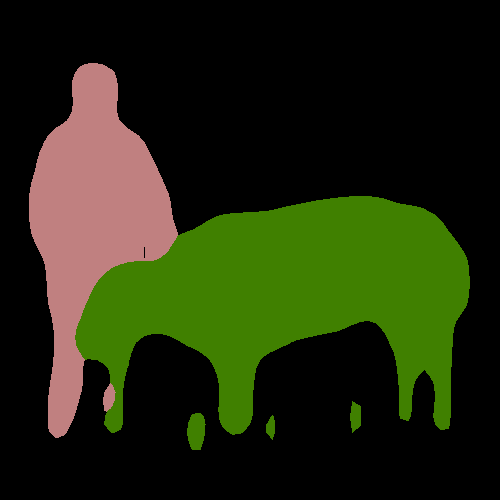
\includegraphics[width=0.16\textwidth]{image/appendix1/5/2011_001159.png} \\
	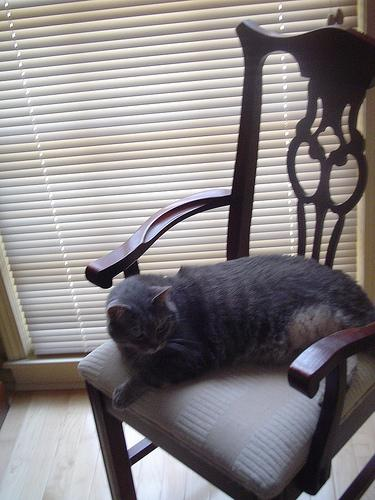
\includegraphics[width=0.16\textwidth]{image/appendix1/2011_000813.jpg}
	
\includegraphics[width=0.16\textwidth]{image/appendix1/2011_000813.png}
	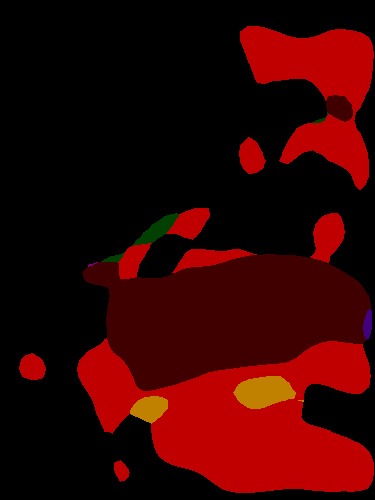
\includegraphics[width=0.16\textwidth]{image/appendix1/1/2011_000813.png}
	
\includegraphics[width=0.16\textwidth]{image/appendix1/3/2011_000813.png}
	
\includegraphics[width=0.16\textwidth]{image/appendix1/5/2011_000813.png} \\
	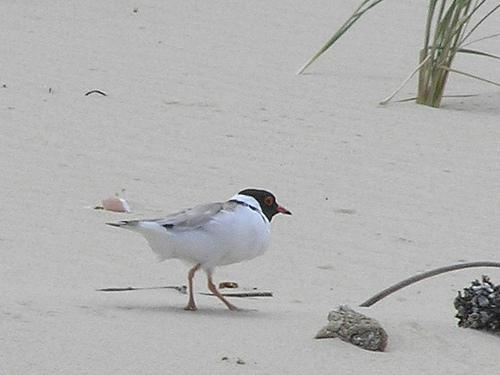
\includegraphics[width=0.16\textwidth]{image/appendix1/2011_003145.jpg}
	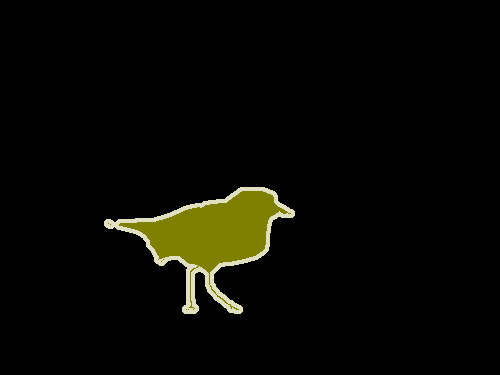
\includegraphics[width=0.16\textwidth]{image/appendix1/2011_003145.png}
	
\includegraphics[width=0.16\textwidth]{image/appendix1/1/2011_003145.png}
	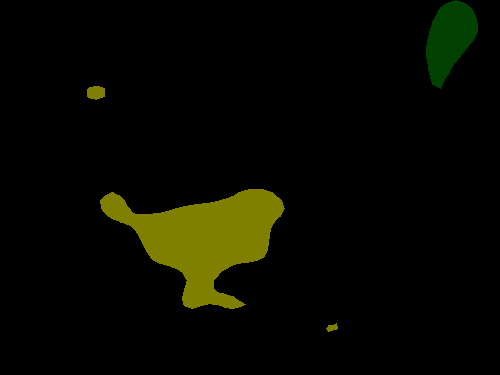
\includegraphics[width=0.16\textwidth]{image/appendix1/3/2011_003145.png}
	
\includegraphics[width=0.16\textwidth]{image/appendix1/5/2011_003145.png} \\
	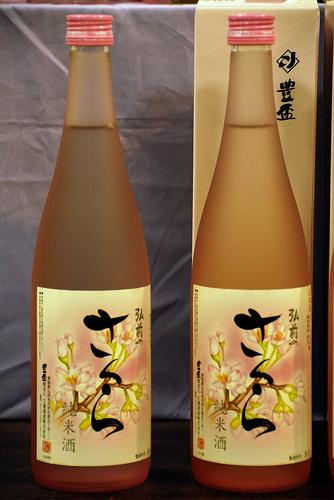
\includegraphics[width=0.16\textwidth]{image/appendix1/2009_004579.jpg}
	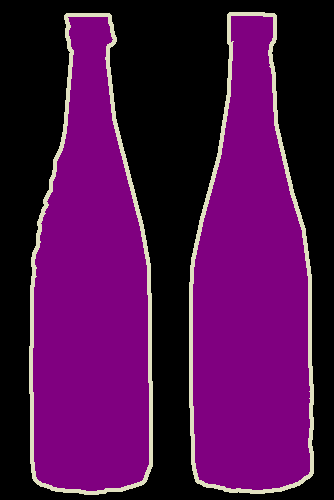
\includegraphics[width=0.16\textwidth]{image/appendix1/2009_004579.png}
	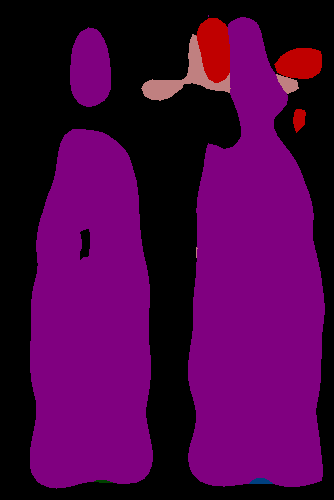
\includegraphics[width=0.16\textwidth]{image/appendix1/1/2009_004579.png}
	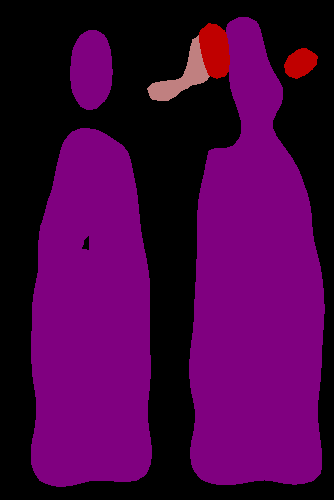
\includegraphics[width=0.16\textwidth]{image/appendix1/3/2009_004579.png}
	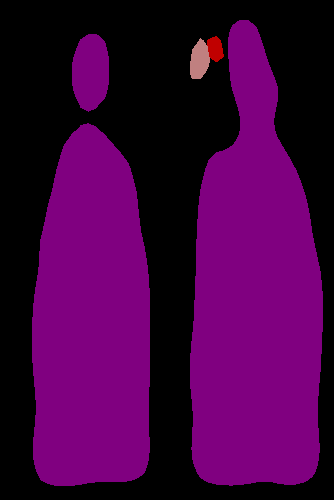
\includegraphics[width=0.16\textwidth]{image/appendix1/5/2009_004579.png} \\
	\color[rgb]{0.9,0.9,0.9}\bfseries
	\begin{tabular}{*{7}{>{\centering\arraybackslash}p{0.10\textwidth}}}
		\hline
		\cellcolor[rgb]{0,0,0}  背景                 & \cellcolor[rgb]{0.5020,0,0} 飞机         & \cellcolor[rgb]{0,0.5020,0} 自行车 & \cellcolor[rgb]{0.5020,0.5020,0} 鸟 & \cellcolor[rgb]{0,0,0.5020} 船        & \cellcolor[rgb]{0.5020,0,0.5020} 瓶子 & \cellcolor[rgb]{0,0.5020,0.5020} 大巴
		\\
		\hline
		\cellcolor[rgb]{0.5020,0.5020,0.5020} 汽车   & \cellcolor[rgb]{0.2510,0,0} 猫           & \cellcolor[rgb]{0.7529,0,0} 椅子   & \cellcolor[rgb]{0.2510,0.5020,0} 牛 & \cellcolor[rgb]{0.7529,0.5020,0} 桌子 & \cellcolor[rgb]{0.2510,0,0.5020} 狗   & \cellcolor[rgb]{0.7529,0,0.5020} 马   \\
		\hline
		\cellcolor[rgb]{0.2510,0.5020,0.5020} 摩托车 & \cellcolor[rgb]{0.7529,0.5020,0.5020} 人 & \cellcolor[rgb]{0,0.2510,0} 盆栽   & \cellcolor[rgb]{0.5020,0.2510,0} 羊 & \cellcolor[rgb]{0,0.7529,0} 沙发      & \cellcolor[rgb]{0.5020,0.7529,0} 火车 & \cellcolor[rgb]{0,0.2510,0.5020} 电视 \\
		\hline
	\end{tabular}

	\caption{一个配有彩色表格的插图}
\end{figure}

\endinput

    \newclearpage
}

%%
% 致谢
% 谢辞应以简短的文字对课题研究与论文撰写过程中曾直接给予帮助的人员(例如指导教师、答疑教师及其他人员)表示对自己的谢意,这不仅是一种礼貌,也是对他人劳动的尊重,是治学者应当遵循的学术规范。内容限一页。
% modifier: 黄俊杰
% update date: 2017-04-15
%%

\chapter{致谢}

四年时间转眼即逝,青涩而美好的本科生活快告一段落了。回首这段时间,我不仅学习到了很多知识和技能,而且提高了分析和解决问题的能力与养成了一定的科学素养。虽然走过了一些弯路,但更加坚定我后来选择学术研究的道路,实在是获益良多。这一切与老师的教诲和同学们的帮助是分不开的。

首先要感谢的是我的指导老师杜云飞教授。杜云飞教授对整个研究领域有很好的理解,以其渊博的知识和敏锐的洞察力给了我非常有帮助的方向性指导。他严谨的治学态度与辛勤的工作方式也是我学习的榜样,在此向杜云飞教授致以崇高的敬意和衷心的感谢。

其次我要感谢本次项目的合作同学黄俊康师兄。黄俊康师兄有很强的数学功底,实现了算法需要的矩阵生成器和并行广义最小残差过程,大大推进了整个项目的进度。在此表达诚挚的谢意。

然后我要感谢我的家人,正是他们的无私奉献和支持,我才有了不断拼搏的信心和勇气。

最后我要感谢自己的女友,由于她迟迟没有出现在我身边,我得以专心于科研工作,最终取得本次的成果。

\vskip 108pt
\begin{flushright}
	吴坎\makebox[1.2cm]{} \\
	\today
\end{flushright}
    % 致谢
\newclearpage

% \makeGrade      % 成绩评定记录表
\end{document}
